\section{Приложение. Распределение особей {\it Macoma balthica} разного возраста на нижнем горизонте литорали Пала-губы (Кольский залиы, Баренцево море)}
\label{app:Pala_MoranI_ages}


	\begin{figure}[h]
	\begin{minipage}[b]{\linewidth}
	\begin{center}
		Моллюски возрастом 1+
	\end{center}
	\end{minipage}

	\begin{minipage}[b]{.46\linewidth}
%Фигурка в первом ряду слева размер отведенный под весь этот объект \textendash 0.46 от ширины строки
%Параметр [b] означает, что выравнивание этих министраниц будет по нижнему краю
	\begin{center}
		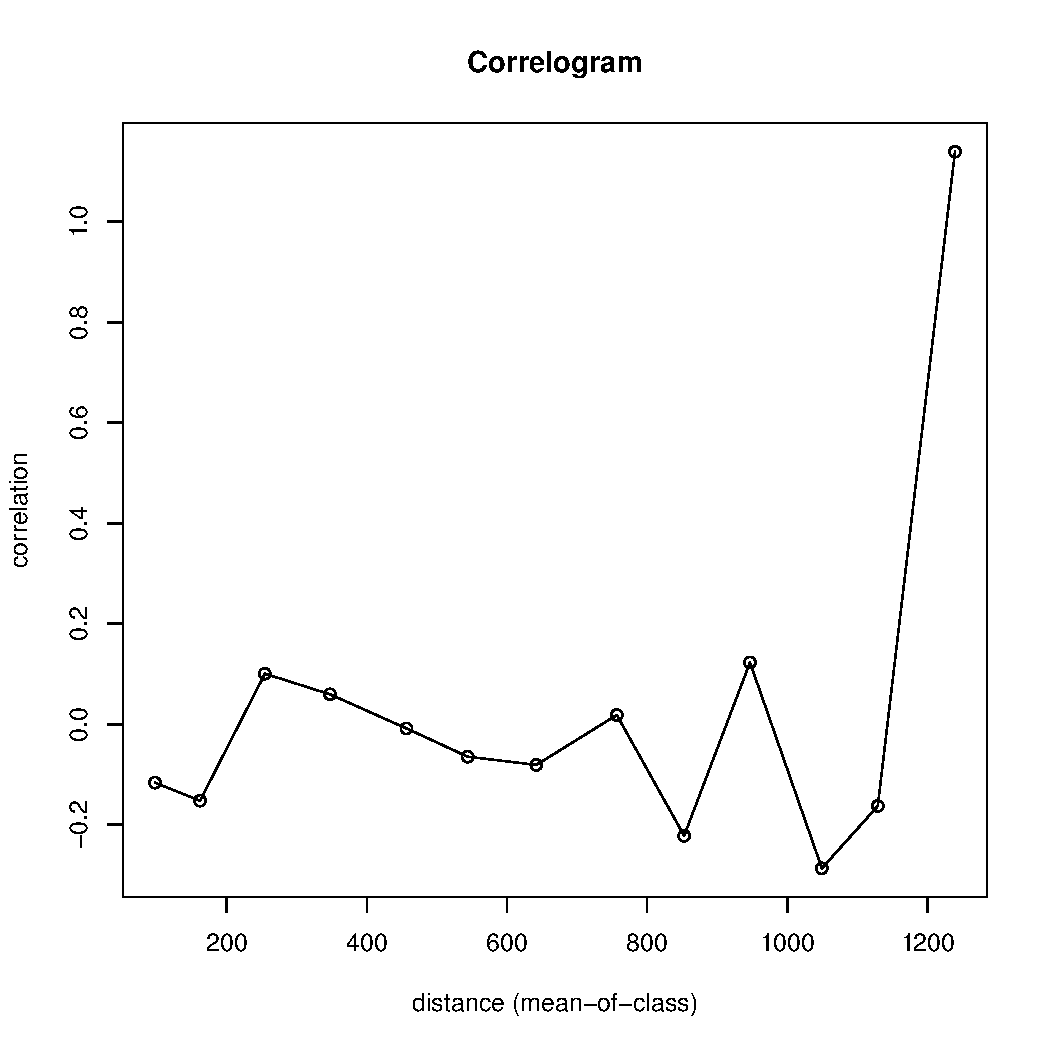
\includegraphics[width=65mm]{../Barenc_Sea/distribution_Moran/Pala_macoma_age_N1_.pdf}
	\end{center}
	\end{minipage}
%
	\hfil %Это пружинка отодвигающая рисунки друг от друга
%
	\begin{minipage}[b]{.46\linewidth}
%Следующий рисунок - первый ряд справа %DUNGEON S_4 \ AB
	\begin{center}
		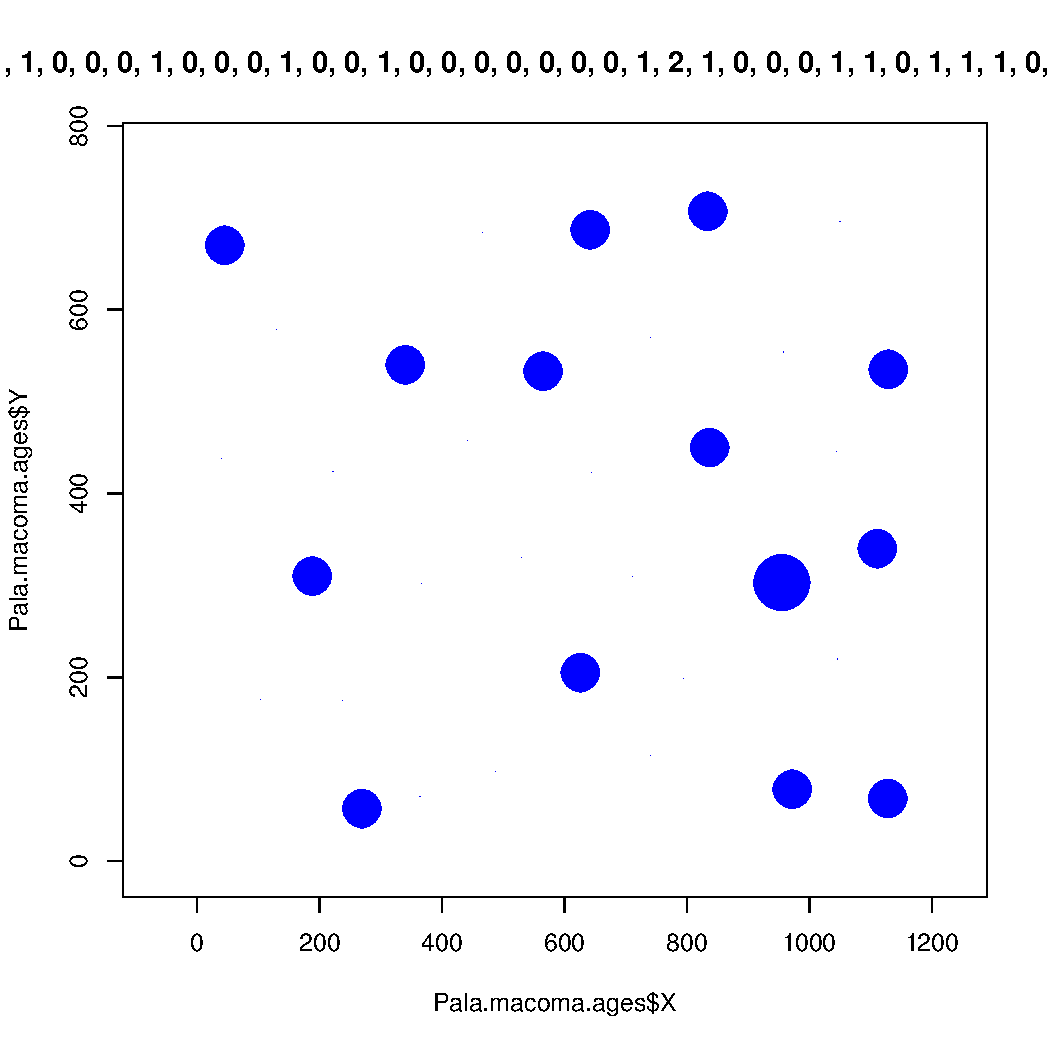
\includegraphics[width=65mm]{../Barenc_Sea/distribution_Moran/Pala_macoma_age_bubb_N1_.pdf}
	\end{center}
	\end{minipage}

	\begin{minipage}[b]{\linewidth}
	\begin{center}
		Моллюски возрастом 2+
	\end{center}
	\end{minipage}

	\begin{minipage}[b]{.46\linewidth}
%Фигурка в первом ряду слева размер отведенный под весь этот объект \textendash 0.46 от ширины строки
%Параметр [b] означает, что выравнивание этих министраниц будет по нижнему краю
	\begin{center}
		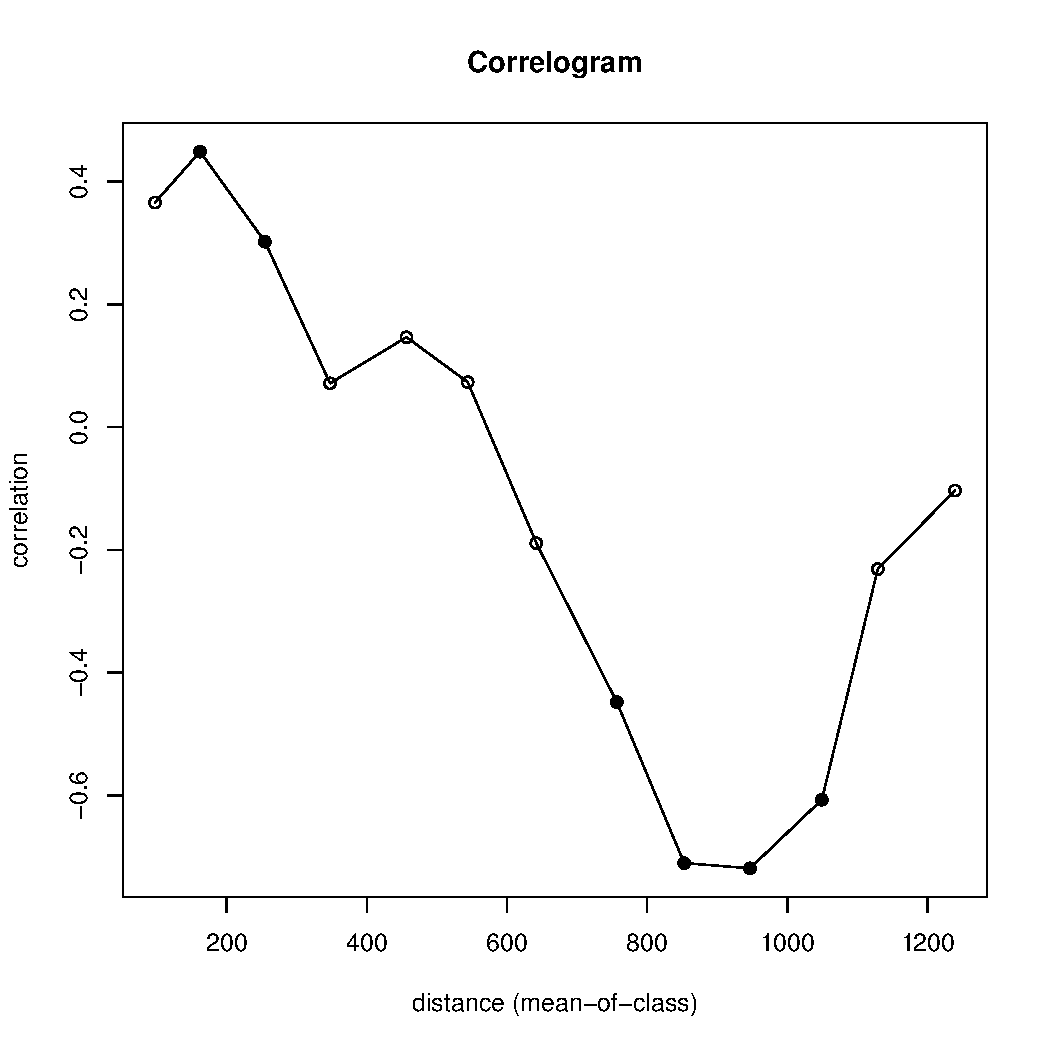
\includegraphics[width=65mm]{../Barenc_Sea/distribution_Moran/Pala_macoma_age_N2_.pdf}
	\end{center}
	\end{minipage}
%
	\hfil %Это пружинка отодвигающая рисунки друг от друга
%
	\begin{minipage}[b]{.46\linewidth}
%Следующий рисунок - первый ряд справа %DUNGEON S_4 \ AB
	\begin{center}
		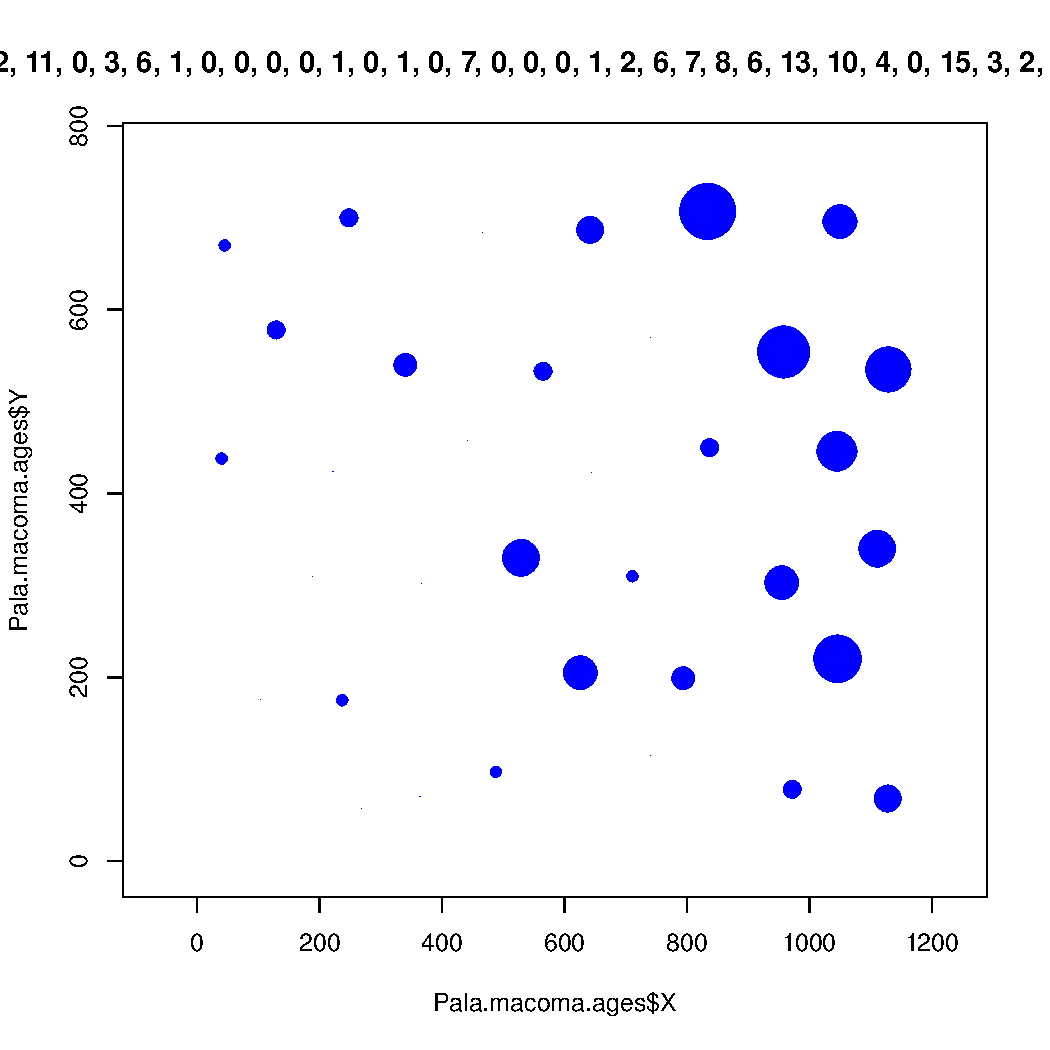
\includegraphics[width=65mm]{../Barenc_Sea/distribution_Moran/Pala_macoma_age_bubb_N2_.pdf}
	\end{center}
	\end{minipage}

%	\caption{Микрораспределение макробентоса на литорали Пала-губы}
%	\label{ris:moransI_Pala}
	\end{figure}




	\begin{figure}[h]

	\begin{minipage}[b]{\linewidth}
	\begin{center}
		Моллюски возрастом 3+
	\end{center}
	\end{minipage}
	
	\begin{minipage}[b]{.46\linewidth}
	%Фигурка в первом ряду слева размер отведенный под весь этот объект \textendash 0.46 от ширины строки
	%Параметр [b] означает, что выравнивание этих министраниц будет по нижнему краю
	\begin{center}
%	{\small N~{\it Cerastoderma edule}}
		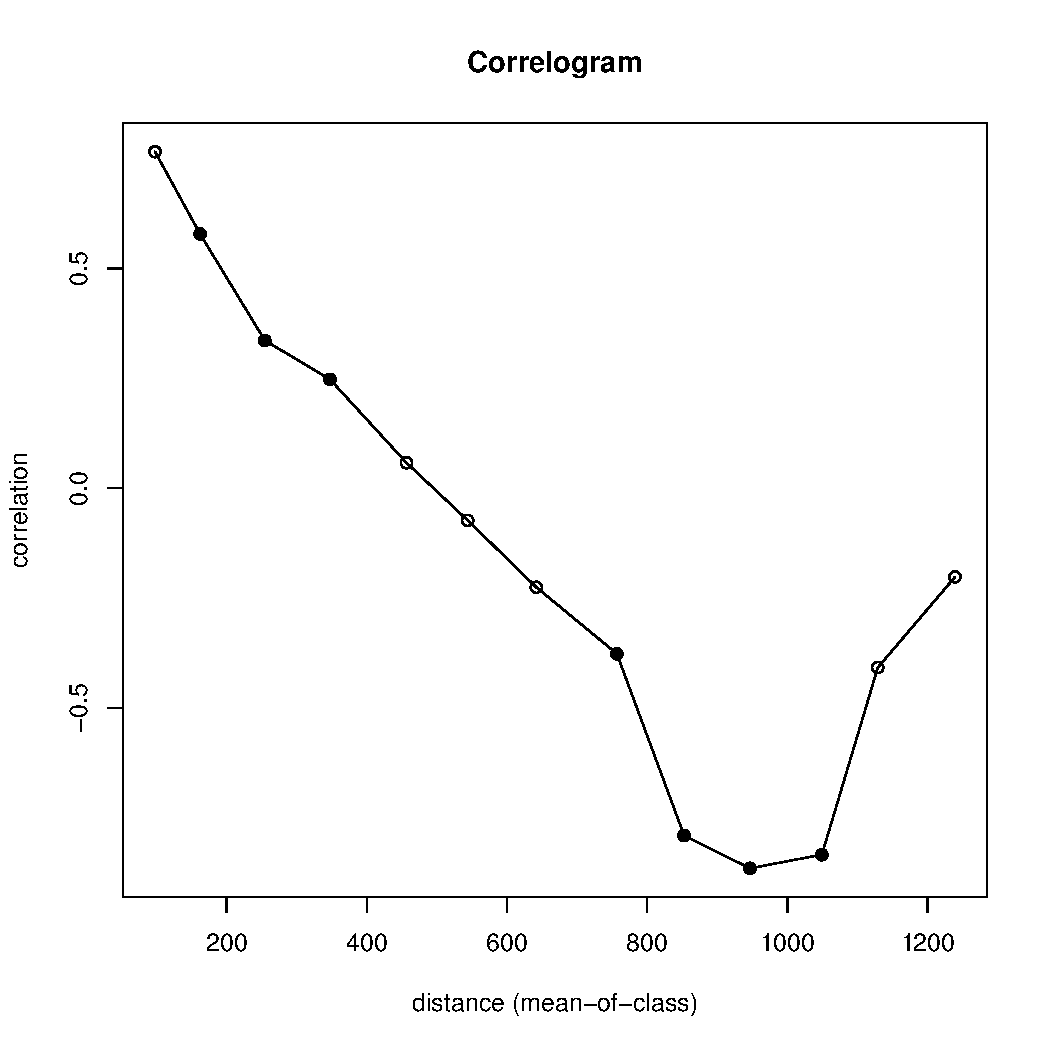
\includegraphics[width=65mm]{../Barenc_Sea/distribution_Moran/Pala_macoma_age_N3_.pdf}
	\end{center}
	\end{minipage}
	%
	\hfil %Это пружинка отодвигающая рисунки друг от друга
	%
	\begin{minipage}[b]{.46\linewidth}
%Следующий рисунок - первый ряд справа %DUNGEON S_4 \ AB
	\begin{center}
		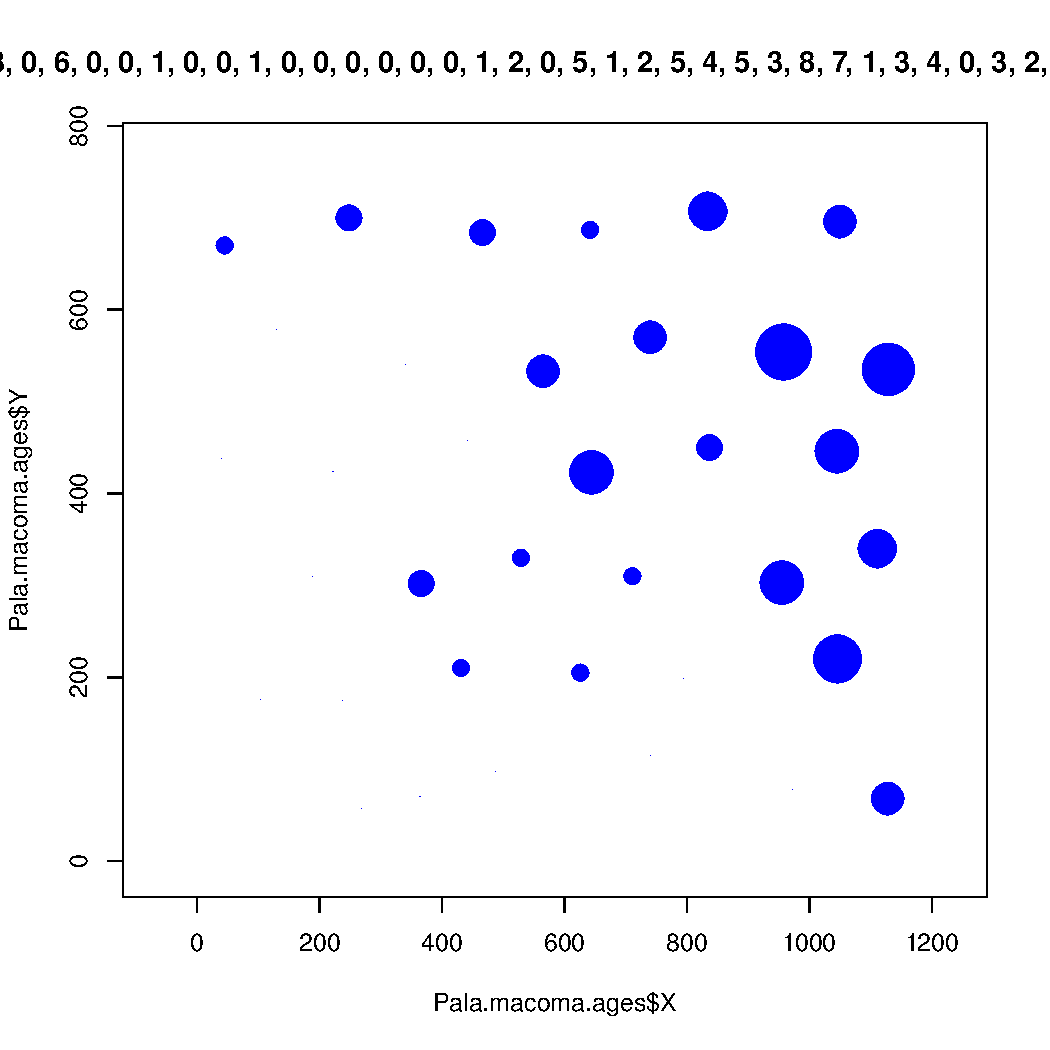
\includegraphics[width=65mm]{../Barenc_Sea/distribution_Moran/Pala_macoma_age_bubb_N3_.pdf}
	\end{center}
	\end{minipage}

	\begin{minipage}[b]{\linewidth}
	\begin{center}
		Моллюски возрастом 4+
	\end{center}
	\end{minipage}

	\begin{minipage}[b]{.46\linewidth}
%Фигурка в первом ряду слева размер отведенный под весь этот объект \textendash 0.46 от ширины строки
%Параметр [b] означает, что выравнивание этих министраниц будет по нижнему краю
	\begin{center}
		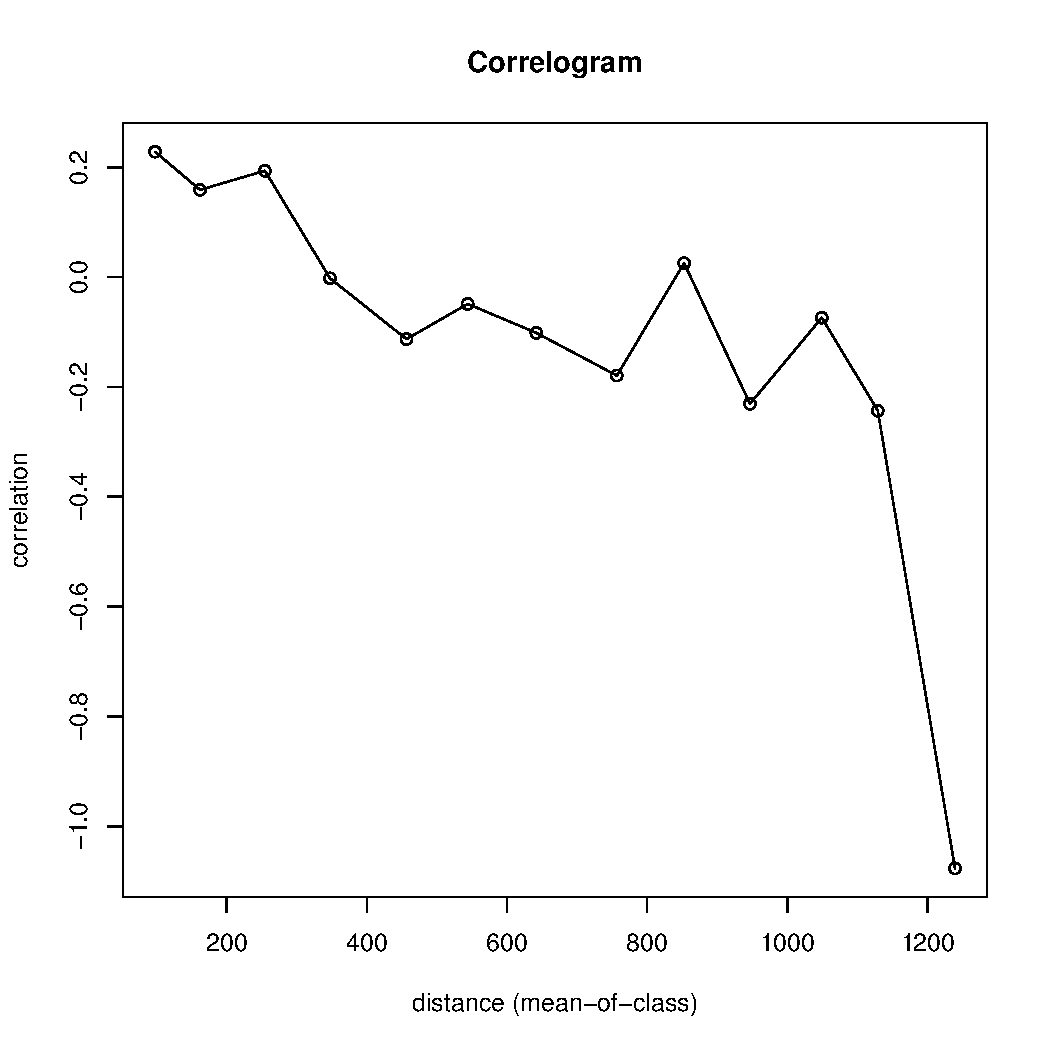
\includegraphics[width=65mm]{../Barenc_Sea/distribution_Moran/Pala_macoma_age_N4_.pdf}
	\end{center}
	\end{minipage}
%
	\hfil %Это пружинка отодвигающая рисунки друг от друга
%
	\begin{minipage}[b]{.46\linewidth}
%Следующий рисунок - первый ряд справа %DUNGEON S_4 \ AB
	\begin{center}
		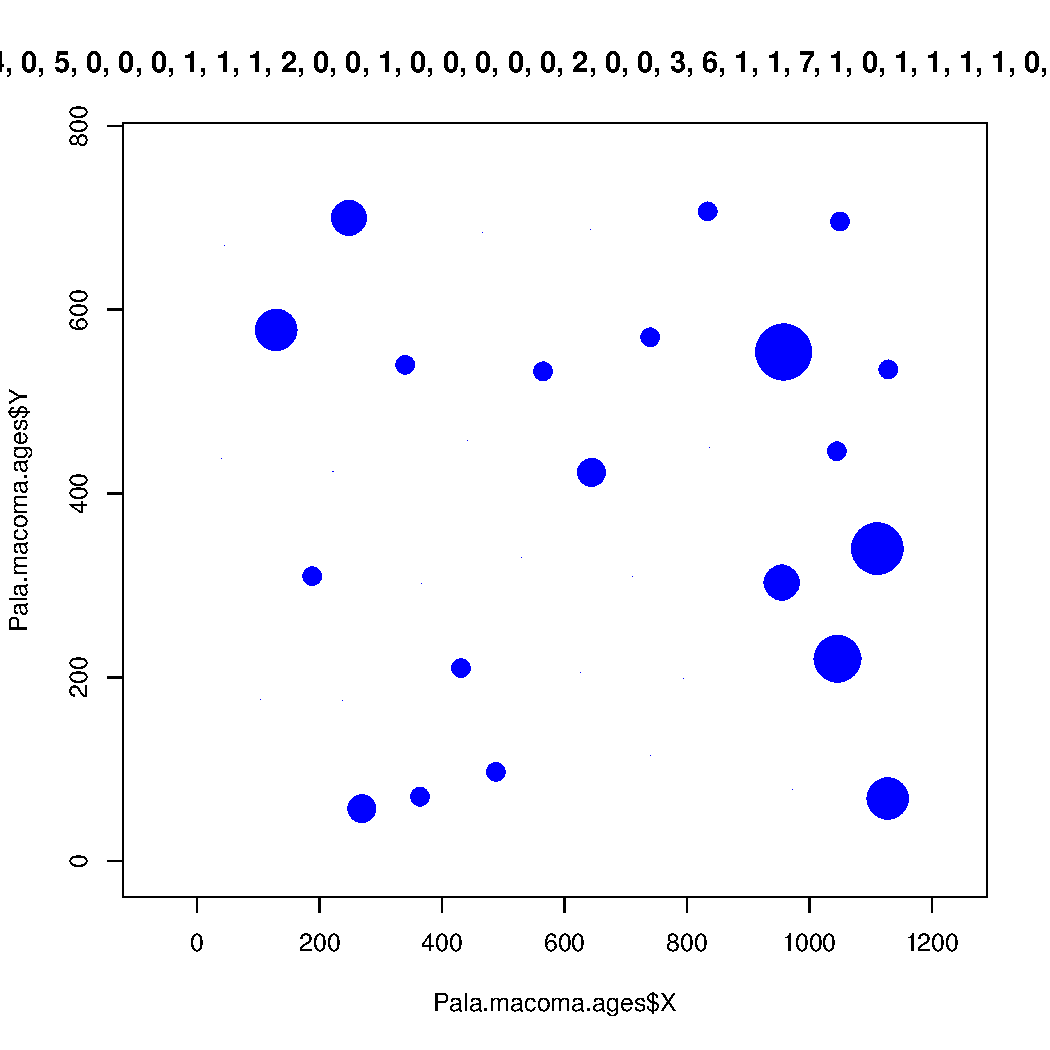
\includegraphics[width=65mm]{../Barenc_Sea/distribution_Moran/Pala_macoma_age_bubb_N4_.pdf}
	\end{center}
	\end{minipage}

	\begin{minipage}[b]{\linewidth}
	\begin{center}
		Моллюски возрастом 5+
	\end{center}
	\end{minipage}
	
	\begin{minipage}[b]{.46\linewidth}
	%Фигурка в первом ряду слева размер отведенный под весь этот объект \textendash 0.46 от ширины строки
	%Параметр [b] означает, что выравнивание этих министраниц будет по нижнему краю
	\begin{center}
%	{\small N~{\it Cerastoderma edule}}
		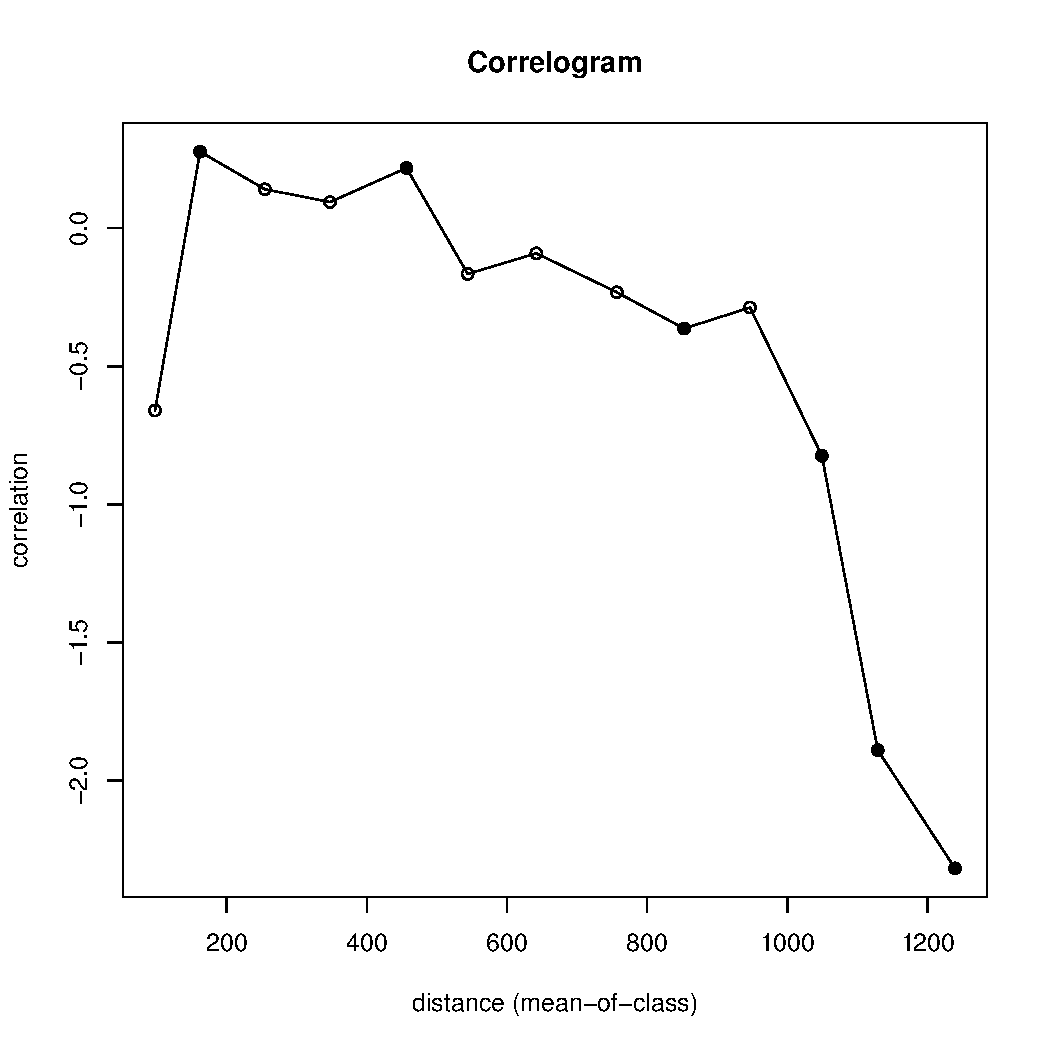
\includegraphics[width=65mm]{../Barenc_Sea/distribution_Moran/Pala_macoma_age_N5_.pdf}
	\end{center}
	\end{minipage}
	%
	\hfil %Это пружинка отодвигающая рисунки друг от друга
	%
	\begin{minipage}[b]{.46\linewidth}
%Следующий рисунок - первый ряд справа %DUNGEON S_4 \ AB
	\begin{center}
		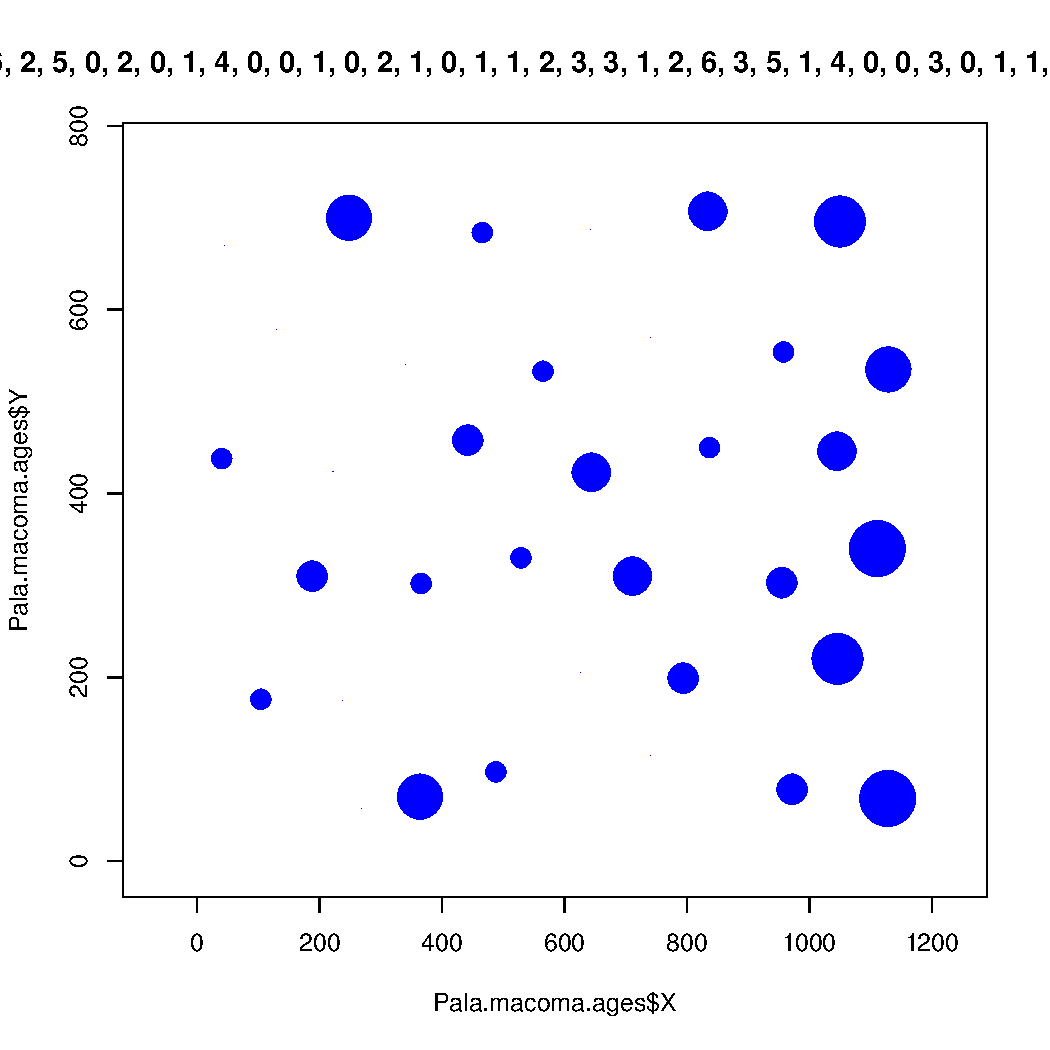
\includegraphics[width=65mm]{../Barenc_Sea/distribution_Moran/Pala_macoma_age_bubb_N5_.pdf}
	\end{center}
	\end{minipage}

%	\caption{Микрораспределение макробентоса на литорали Пала-губы}
%	\label{ris:moransI_Pala}
	\end{figure}




	\begin{figure}[h]

	\begin{minipage}[b]{\linewidth}
	\begin{center}
		Моллюски возрастом 6+
	\end{center}
	\end{minipage}
	
	\begin{minipage}[b]{.46\linewidth}
	%Фигурка в первом ряду слева размер отведенный под весь этот объект \textendash 0.46 от ширины строки
	%Параметр [b] означает, что выравнивание этих министраниц будет по нижнему краю
	\begin{center}
%	{\small N~{\it Cerastoderma edule}}
		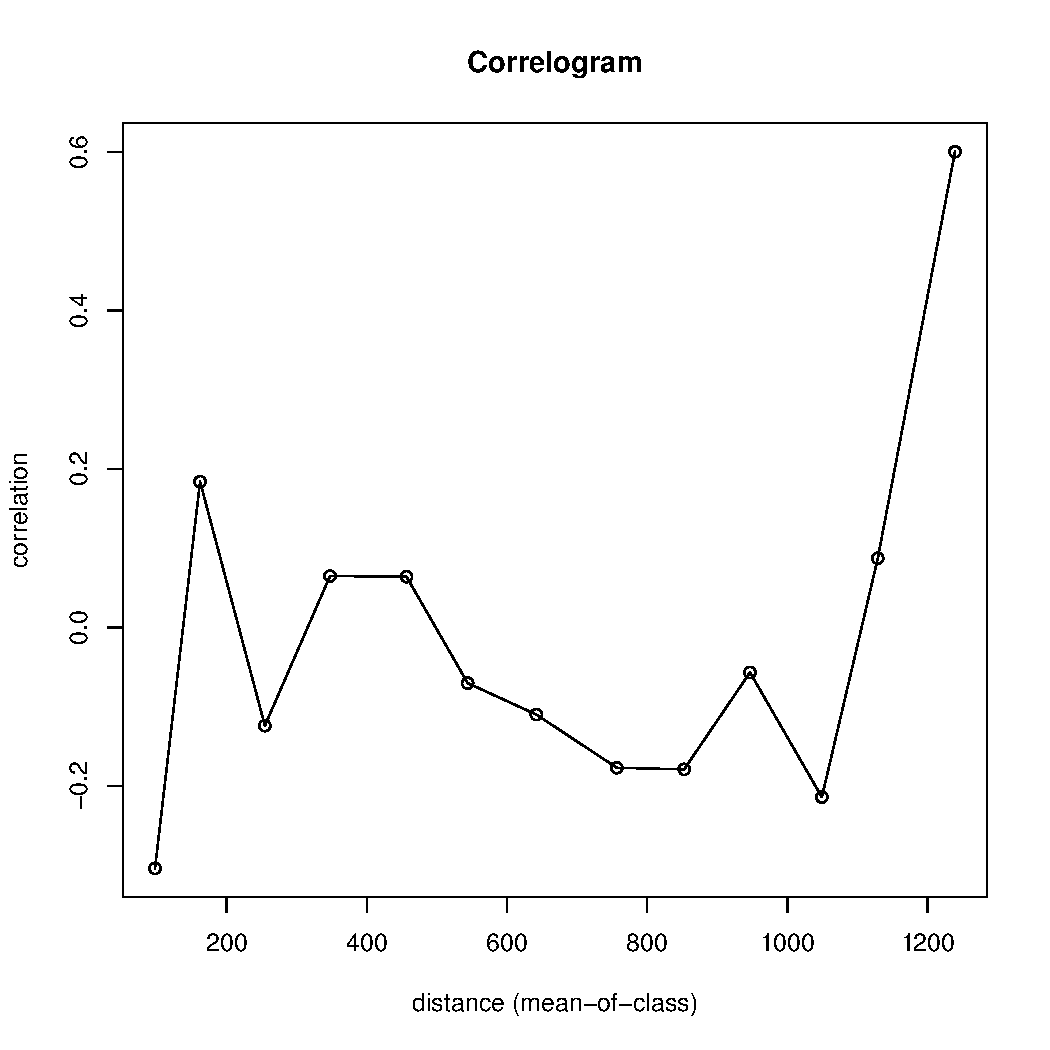
\includegraphics[width=65mm]{../Barenc_Sea/distribution_Moran/Pala_macoma_age_N6_.pdf}
	\end{center}
	\end{minipage}
	%
	\hfil %Это пружинка отодвигающая рисунки друг от друга
	%
	\begin{minipage}[b]{.46\linewidth}
%Следующий рисунок - первый ряд справа %DUNGEON S_4 \ AB
	\begin{center}
		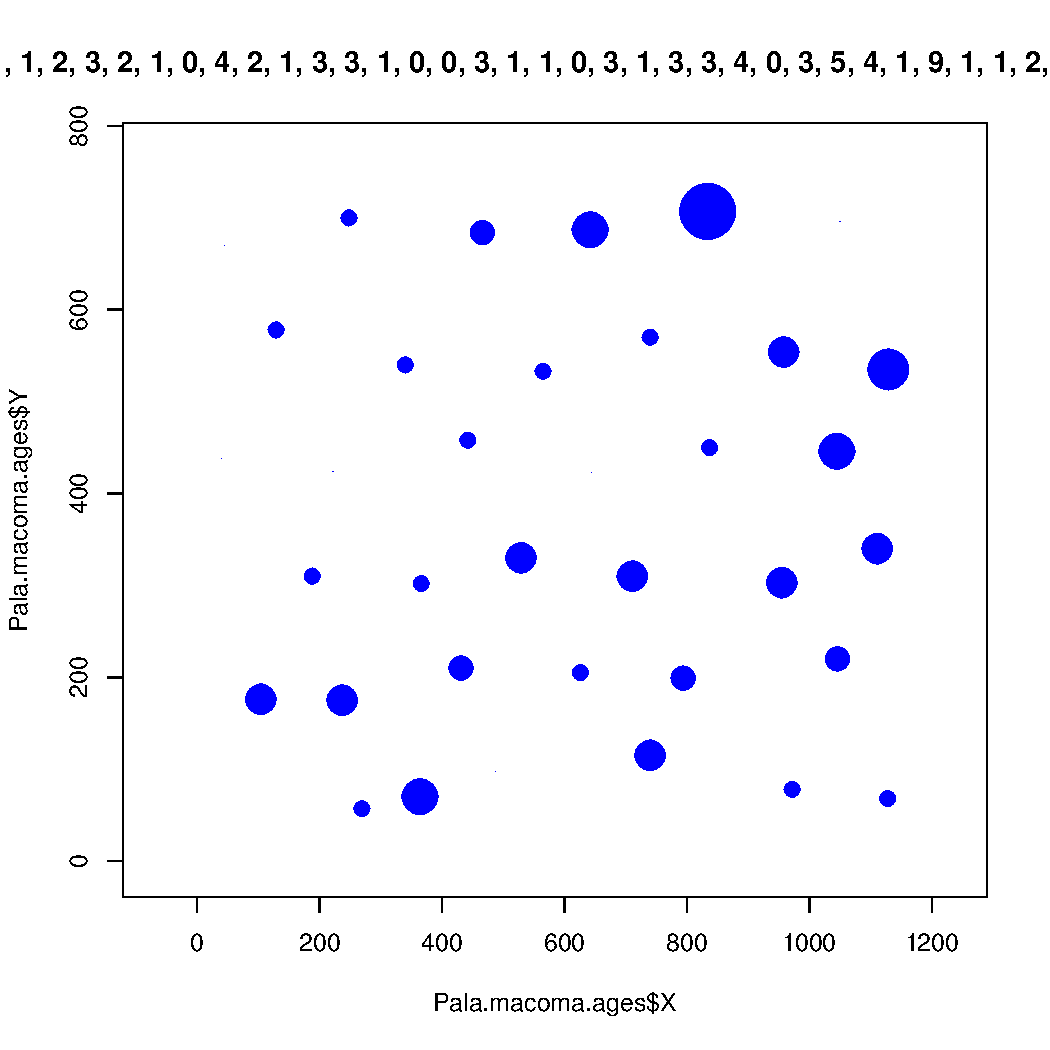
\includegraphics[width=65mm]{../Barenc_Sea/distribution_Moran/Pala_macoma_age_bubb_N6_.pdf}
	\end{center}
	\end{minipage}

	\begin{minipage}[b]{\linewidth}
	\begin{center}
		Моллюски возрастом 7+
	\end{center}
	\end{minipage}

	\begin{minipage}[b]{.46\linewidth}
%Фигурка в первом ряду слева размер отведенный под весь этот объект \textendash 0.46 от ширины строки
%Параметр [b] означает, что выравнивание этих министраниц будет по нижнему краю
	\begin{center}
		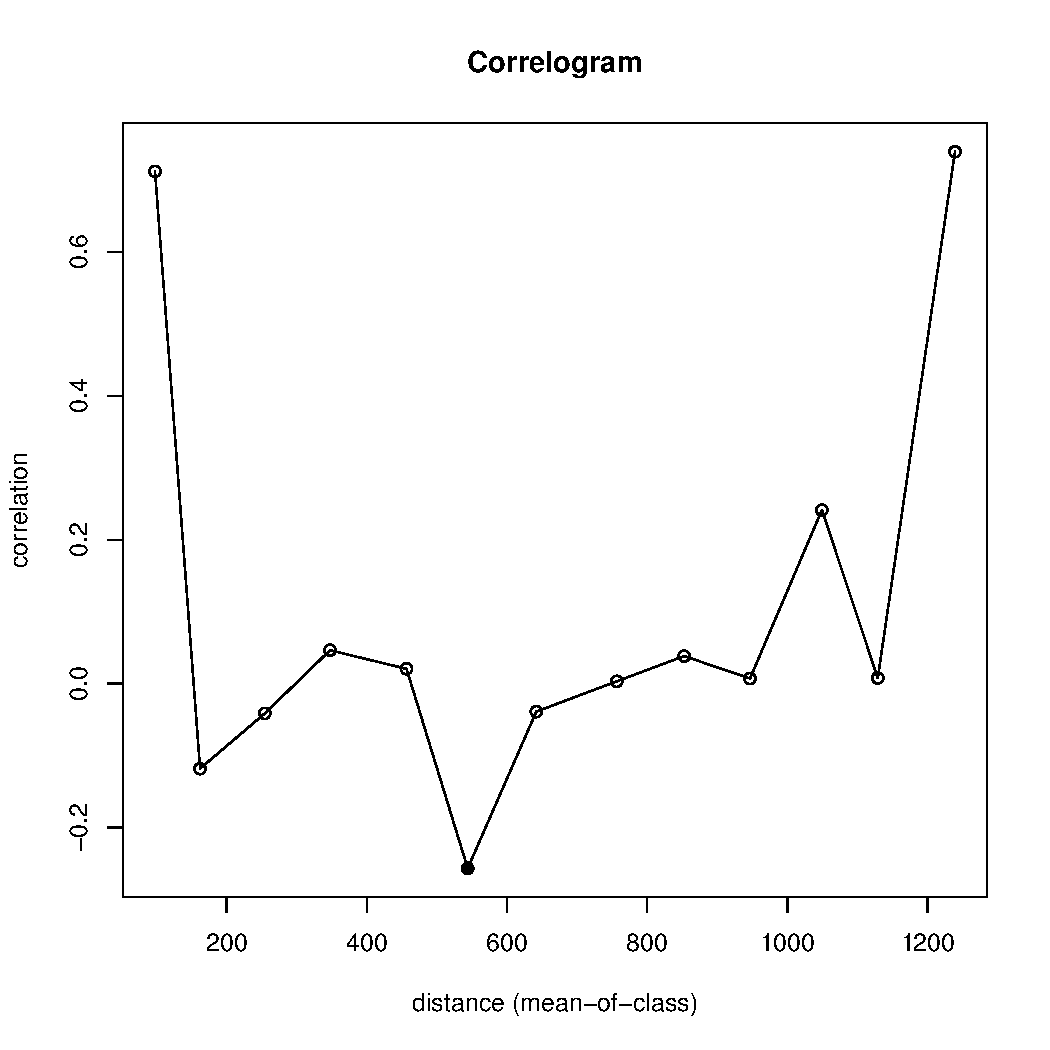
\includegraphics[width=65mm]{../Barenc_Sea/distribution_Moran/Pala_macoma_age_N7_.pdf}
	\end{center}
	\end{minipage}
%
	\hfil %Это пружинка отодвигающая рисунки друг от друга
%
	\begin{minipage}[b]{.46\linewidth}
%Следующий рисунок - первый ряд справа %DUNGEON S_4 \ AB
	\begin{center}
		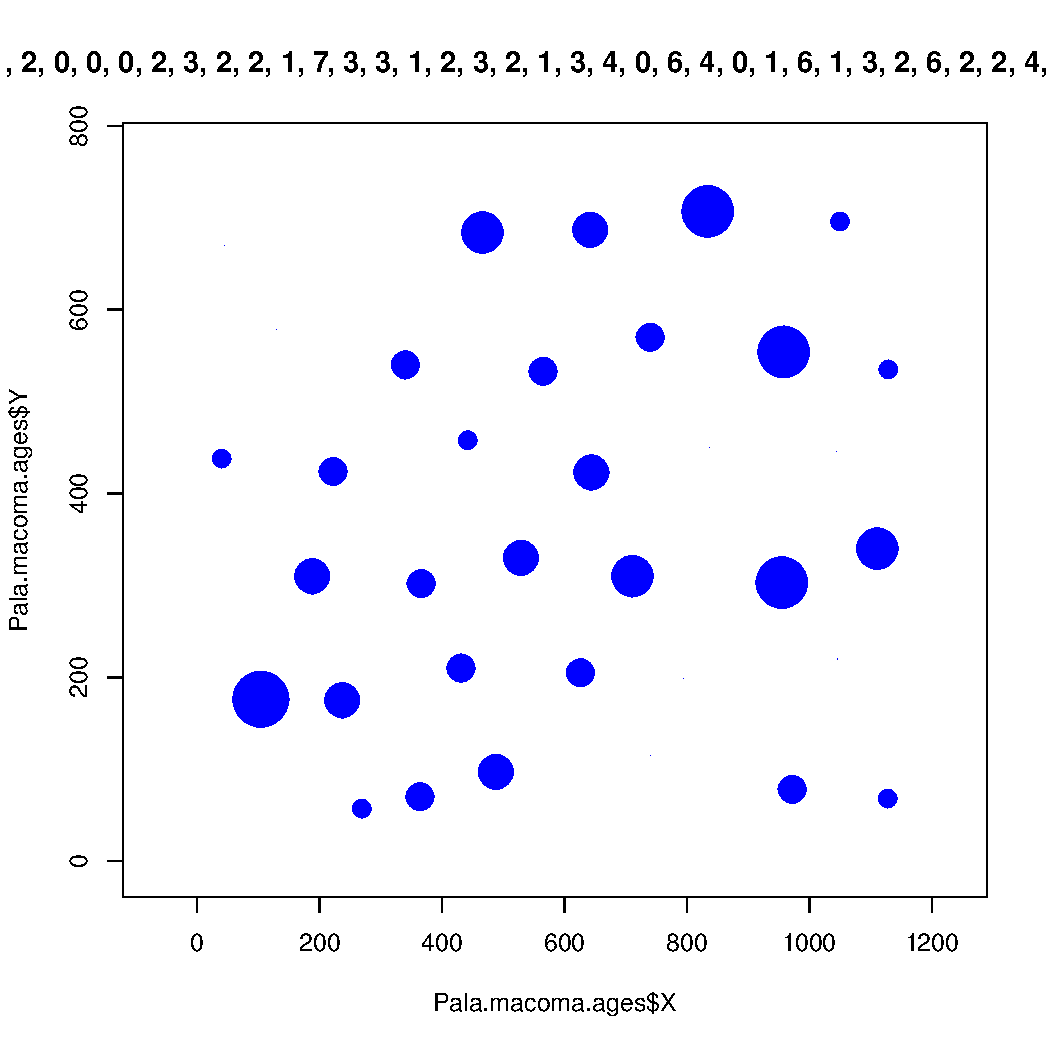
\includegraphics[width=65mm]{../Barenc_Sea/distribution_Moran/Pala_macoma_age_bubb_N7_.pdf}
	\end{center}
	\end{minipage}

	\begin{minipage}[b]{\linewidth}
	\begin{center}
		Моллюски возрастом 8+
	\end{center}
	\end{minipage}
	
	\begin{minipage}[b]{.46\linewidth}
	%Фигурка в первом ряду слева размер отведенный под весь этот объект \textendash 0.46 от ширины строки
	%Параметр [b] означает, что выравнивание этих министраниц будет по нижнему краю
	\begin{center}
%	{\small N~{\it Cerastoderma edule}}
		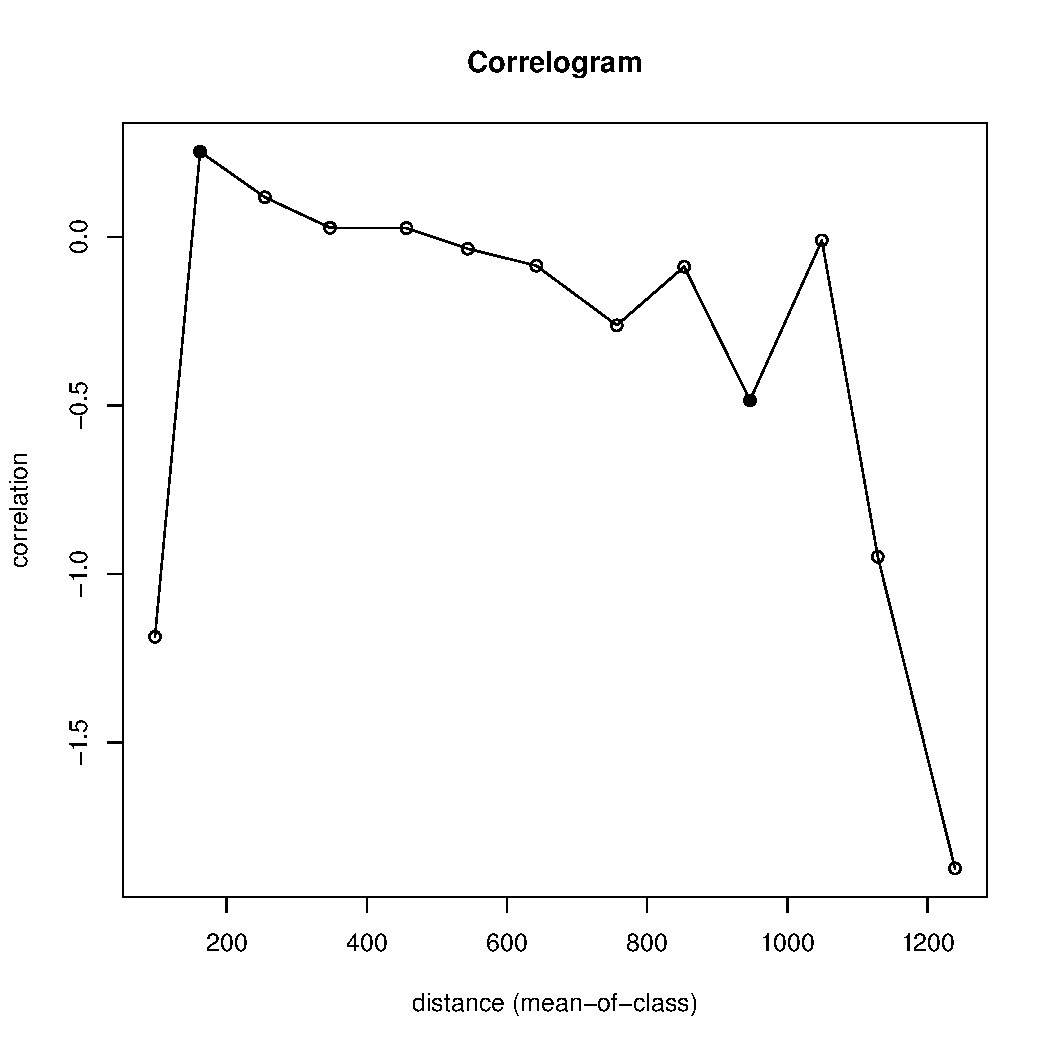
\includegraphics[width=65mm]{../Barenc_Sea/distribution_Moran/Pala_macoma_age_N8_.pdf}
	\end{center}
	\end{minipage}
	%
	\hfil %Это пружинка отодвигающая рисунки друг от друга
	%
	\begin{minipage}[b]{.46\linewidth}
%Следующий рисунок - первый ряд справа %DUNGEON S_4 \ AB
	\begin{center}
		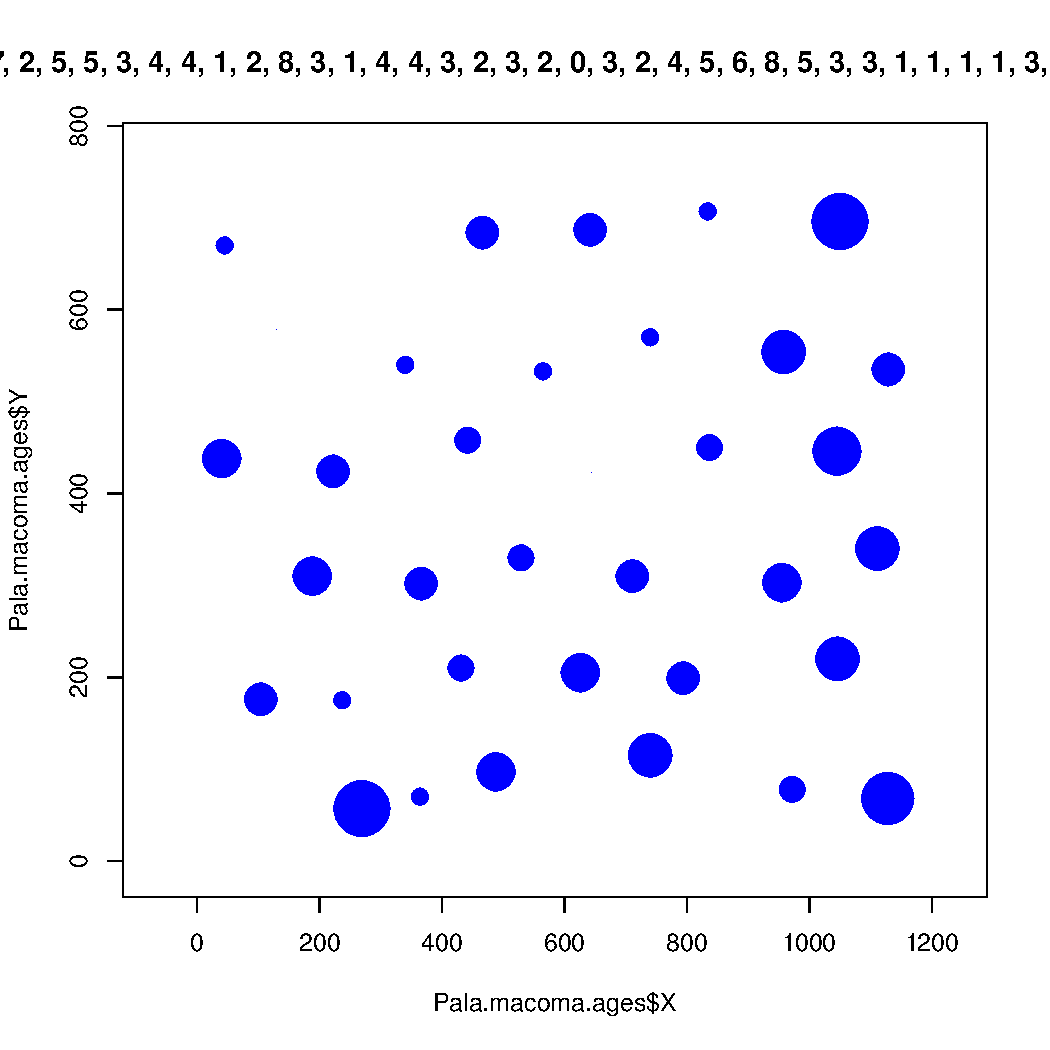
\includegraphics[width=65mm]{../Barenc_Sea/distribution_Moran/Pala_macoma_age_bubb_N8_.pdf}
	\end{center}
	\end{minipage}

%	\caption{Микрораспределение макробентоса на литорали Пала-губы}
%	\label{ris:moransI_Pala}
	\end{figure}




	\begin{figure}[h]

	\begin{minipage}[b]{\linewidth}
	\begin{center}
		Моллюски возрастом 9+
	\end{center}
	\end{minipage}
	
	\begin{minipage}[b]{.46\linewidth}
	%Фигурка в первом ряду слева размер отведенный под весь этот объект \textendash 0.46 от ширины строки
	%Параметр [b] означает, что выравнивание этих министраниц будет по нижнему краю
	\begin{center}
%	{\small N~{\it Cerastoderma edule}}
		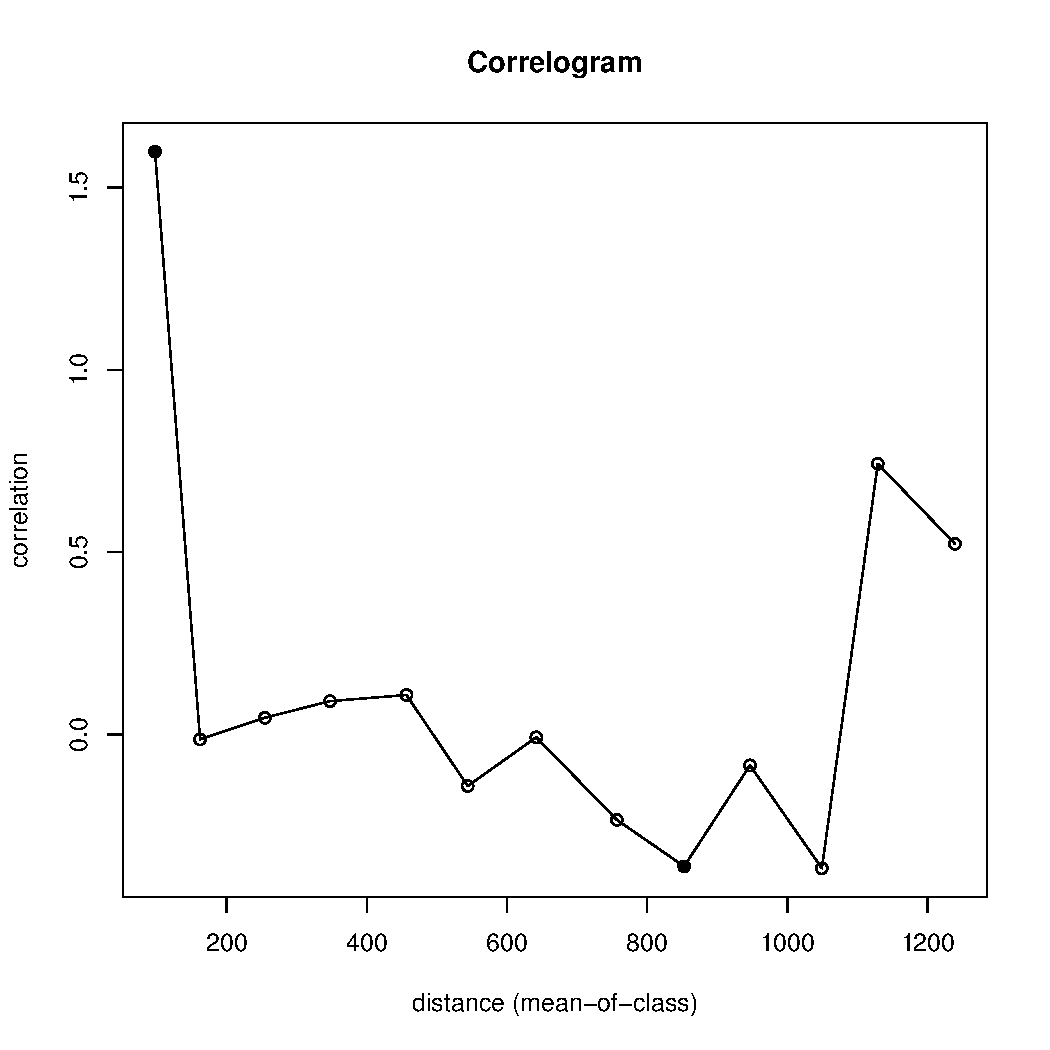
\includegraphics[width=65mm]{../Barenc_Sea/distribution_Moran/Pala_macoma_age_N9_.pdf}
	\end{center}
	\end{minipage}
	%
	\hfil %Это пружинка отодвигающая рисунки друг от друга
	%
	\begin{minipage}[b]{.46\linewidth}
%Следующий рисунок - первый ряд справа %DUNGEON S_4 \ AB
	\begin{center}
		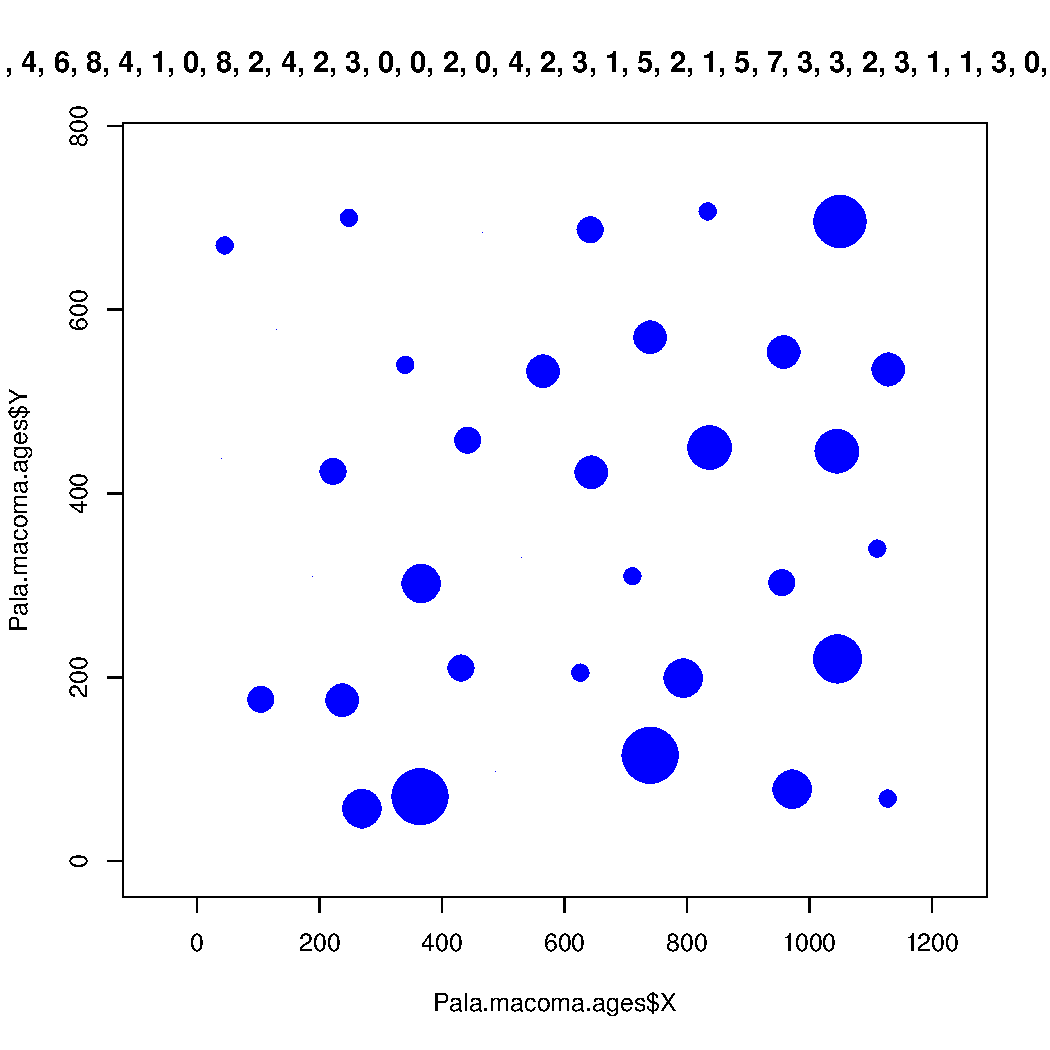
\includegraphics[width=65mm]{../Barenc_Sea/distribution_Moran/Pala_macoma_age_bubb_N9_.pdf}
	\end{center}
	\end{minipage}

	\begin{minipage}[b]{\linewidth}
	\begin{center}
		Моллюски возрастом 10+
	\end{center}
	\end{minipage}

	\begin{minipage}[b]{.46\linewidth}
%Фигурка в первом ряду слева размер отведенный под весь этот объект \textendash 0.46 от ширины строки
%Параметр [b] означает, что выравнивание этих министраниц будет по нижнему краю
	\begin{center}
		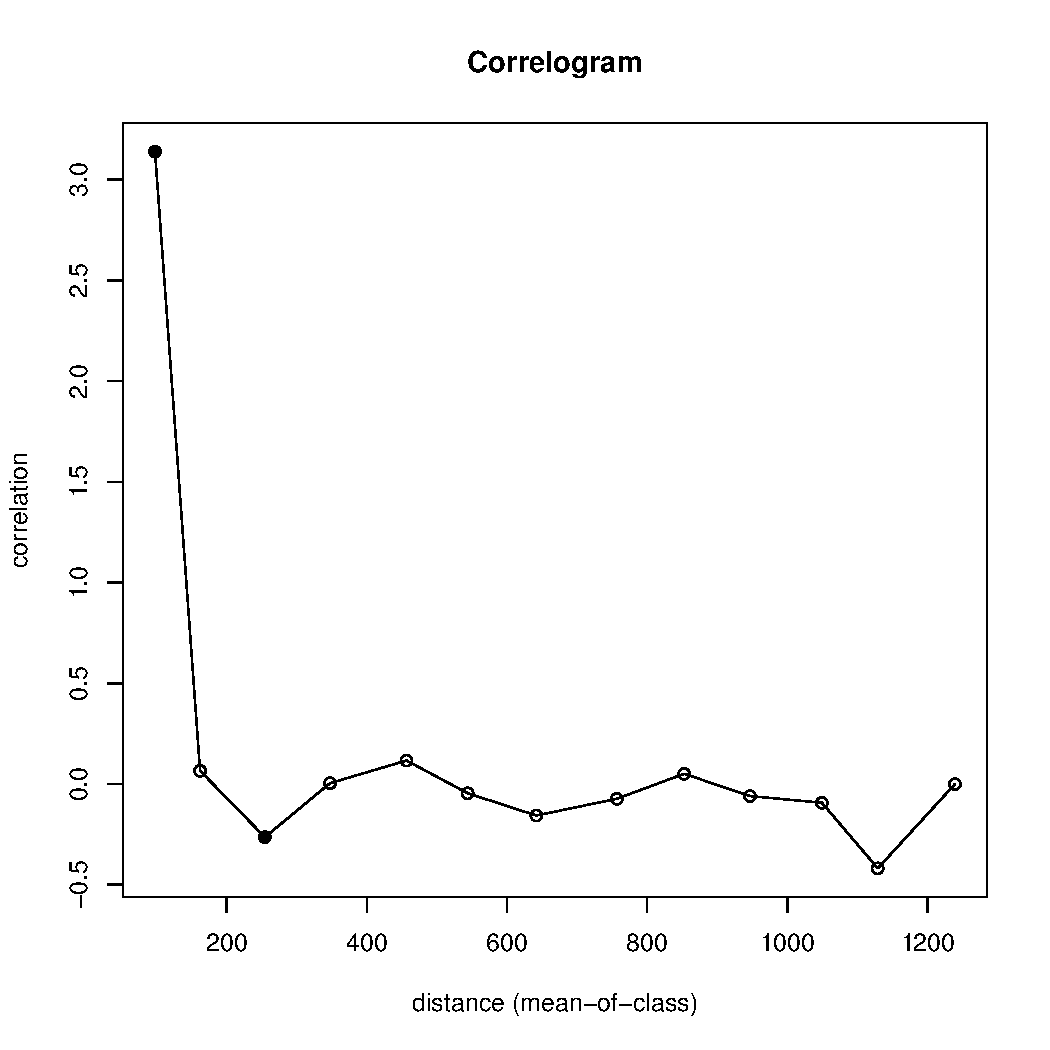
\includegraphics[width=65mm]{../Barenc_Sea/distribution_Moran/Pala_macoma_age_N10_.pdf}
	\end{center}
	\end{minipage}
%
	\hfil %Это пружинка отодвигающая рисунки друг от друга
%
	\begin{minipage}[b]{.46\linewidth}
%Следующий рисунок - первый ряд справа %DUNGEON S_4 \ AB
	\begin{center}
		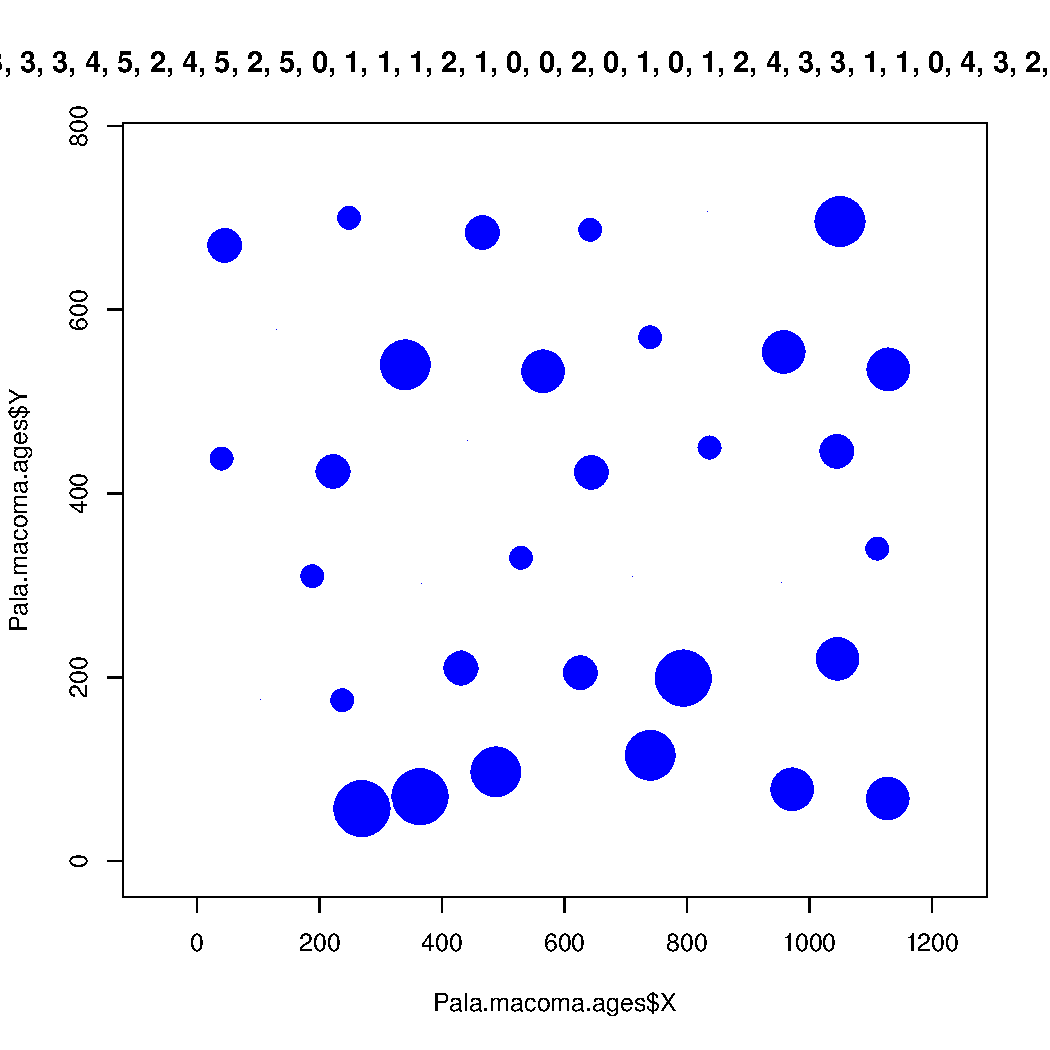
\includegraphics[width=65mm]{../Barenc_Sea/distribution_Moran/Pala_macoma_age_bubb_N10_.pdf}
	\end{center}
	\end{minipage}

	\begin{minipage}[b]{\linewidth}
	\begin{center}
		Моллюски возрастом 11+
	\end{center}
	\end{minipage}
	
	\begin{minipage}[b]{.46\linewidth}
	%Фигурка в первом ряду слева размер отведенный под весь этот объект \textendash 0.46 от ширины строки
	%Параметр [b] означает, что выравнивание этих министраниц будет по нижнему краю
	\begin{center}
%	{\small N~{\it Cerastoderma edule}}
		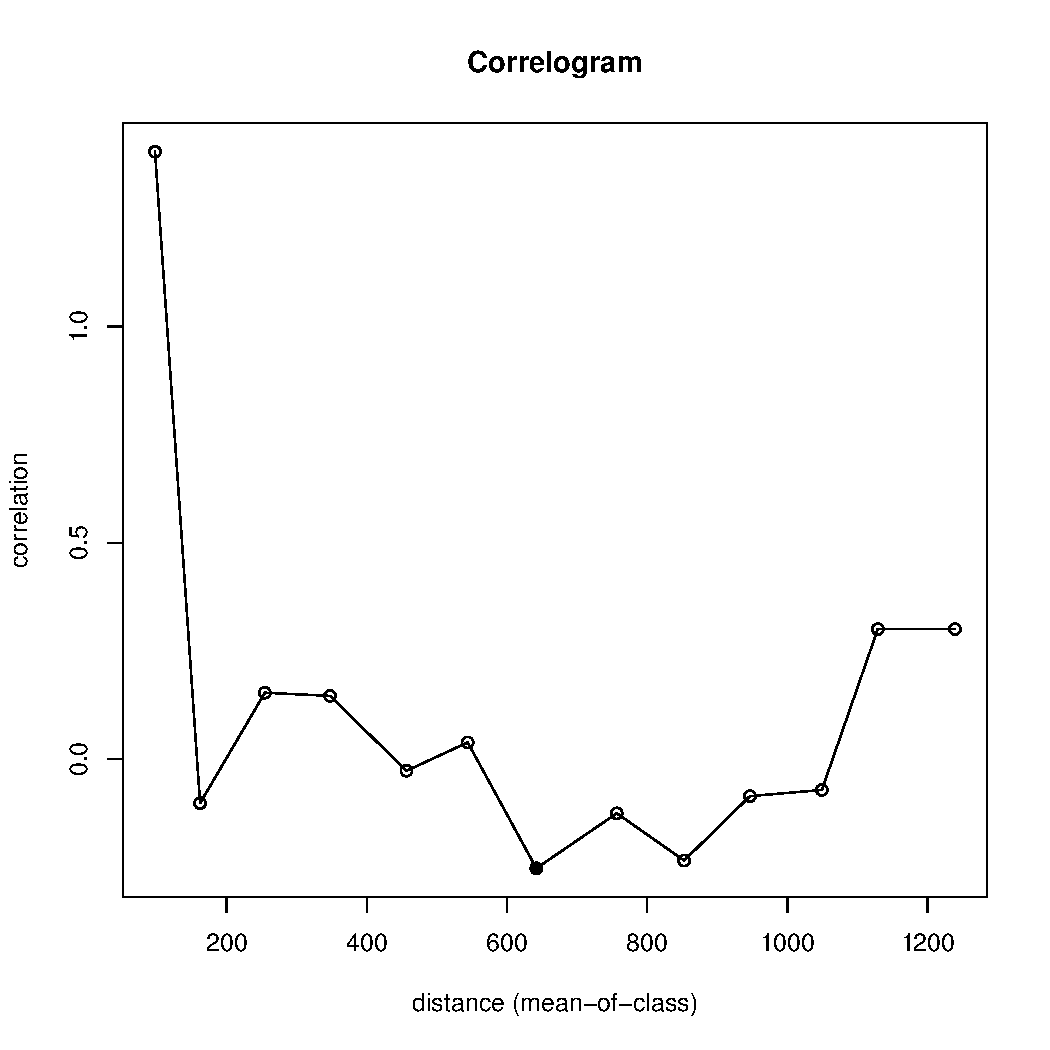
\includegraphics[width=65mm]{../Barenc_Sea/distribution_Moran/Pala_macoma_age_N11_.pdf}
	\end{center}
	\end{minipage}
	%
	\hfil %Это пружинка отодвигающая рисунки друг от друга
	%
	\begin{minipage}[b]{.46\linewidth}
%Следующий рисунок - первый ряд справа %DUNGEON S_4 \ AB
	\begin{center}
		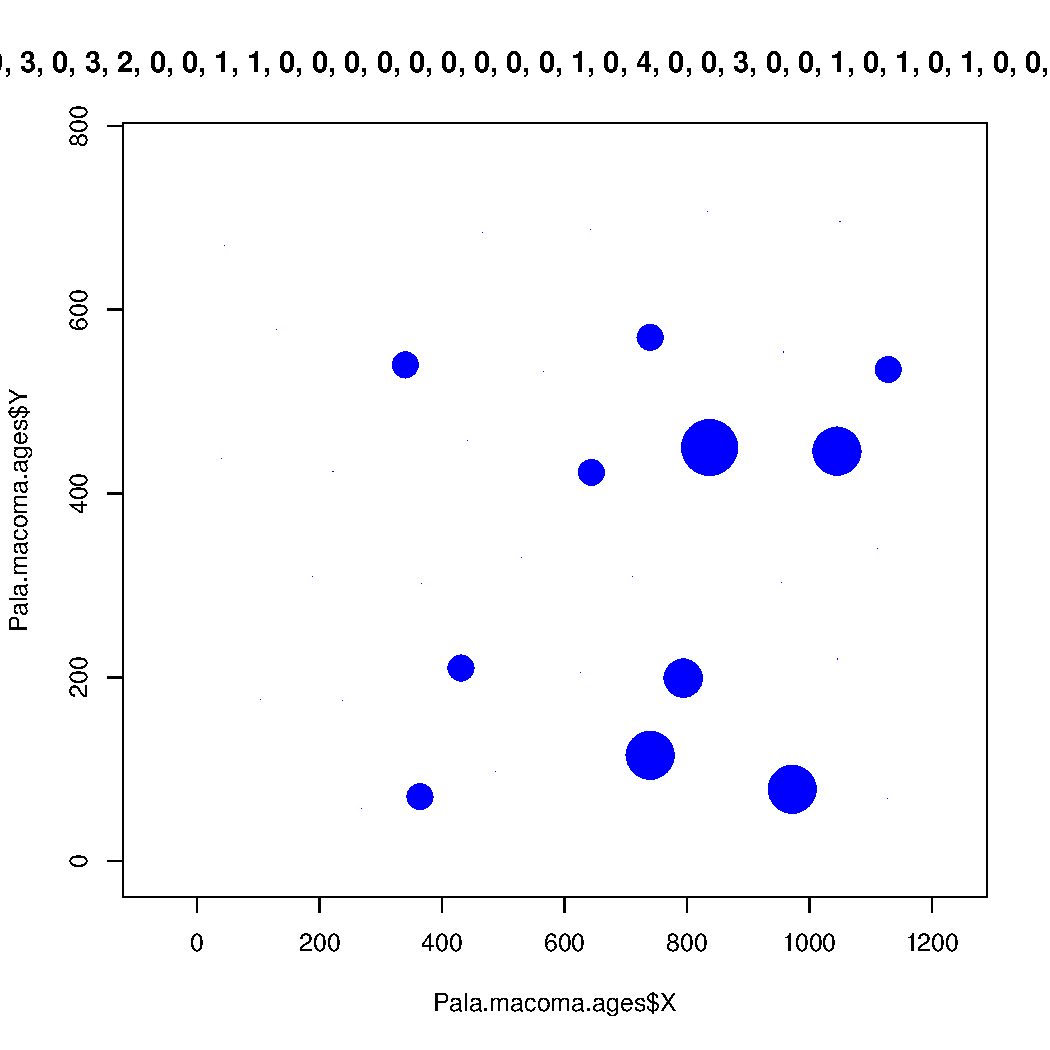
\includegraphics[width=65mm]{../Barenc_Sea/distribution_Moran/Pala_macoma_age_bubb_N11_.pdf}
	\end{center}
	\end{minipage}

%	\caption{Микрораспределение макробентоса на литорали Пала-губы}
%	\label{ris:moransI_Pala}
	\end{figure}




	\begin{figure}[h]

	\begin{minipage}[b]{\linewidth}
	\begin{center}
		Моллюски возрастом 12+
	\end{center}
	\end{minipage}
	
	\begin{minipage}[b]{.46\linewidth}
	%Фигурка в первом ряду слева размер отведенный под весь этот объект \textendash 0.46 от ширины строки
	%Параметр [b] означает, что выравнивание этих министраниц будет по нижнему краю
	\begin{center}
%	{\small N~{\it Cerastoderma edule}}
		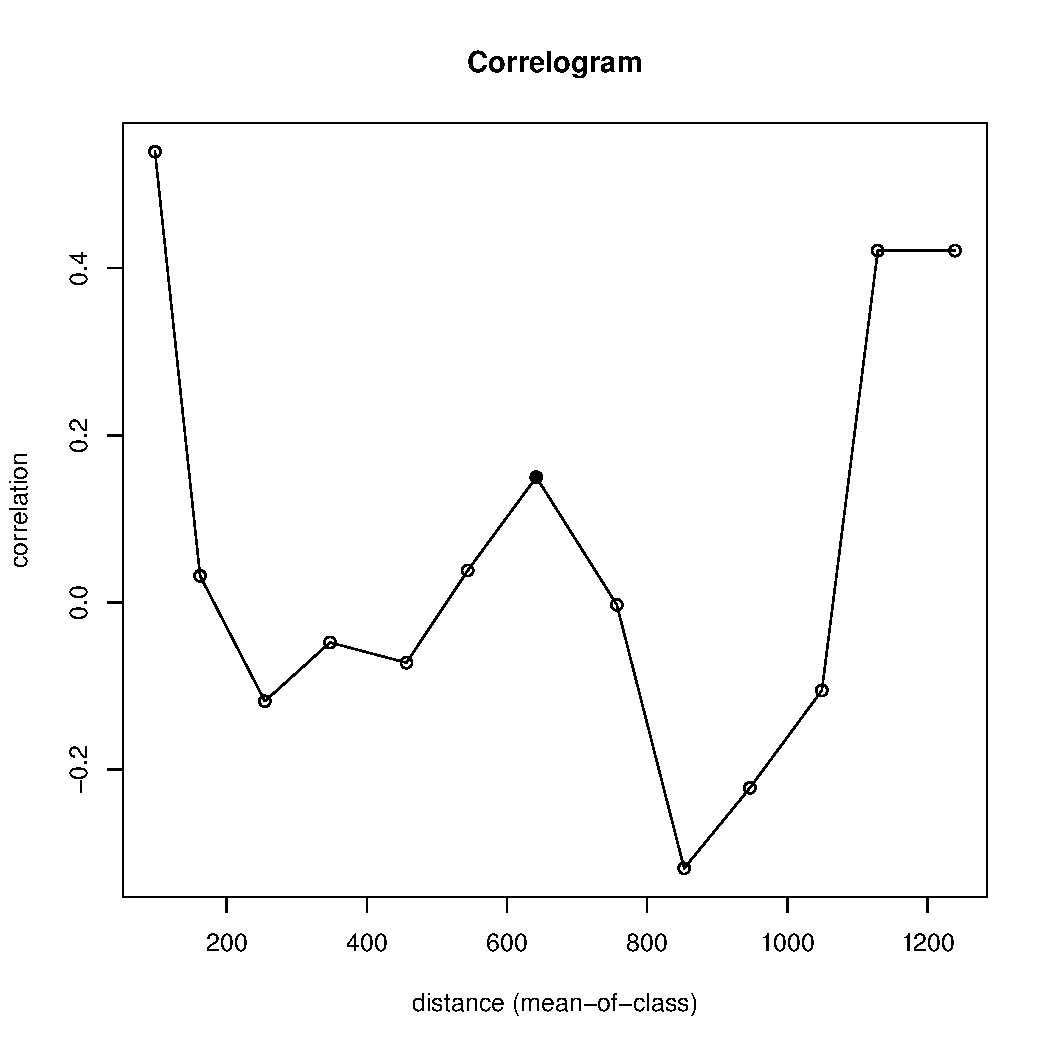
\includegraphics[width=65mm]{../Barenc_Sea/distribution_Moran/Pala_macoma_age_N12_.pdf}
	\end{center}
	\end{minipage}
	%
	\hfil %Это пружинка отодвигающая рисунки друг от друга
	%
	\begin{minipage}[b]{.46\linewidth}
%Следующий рисунок - первый ряд справа %DUNGEON S_4 \ AB
	\begin{center}
		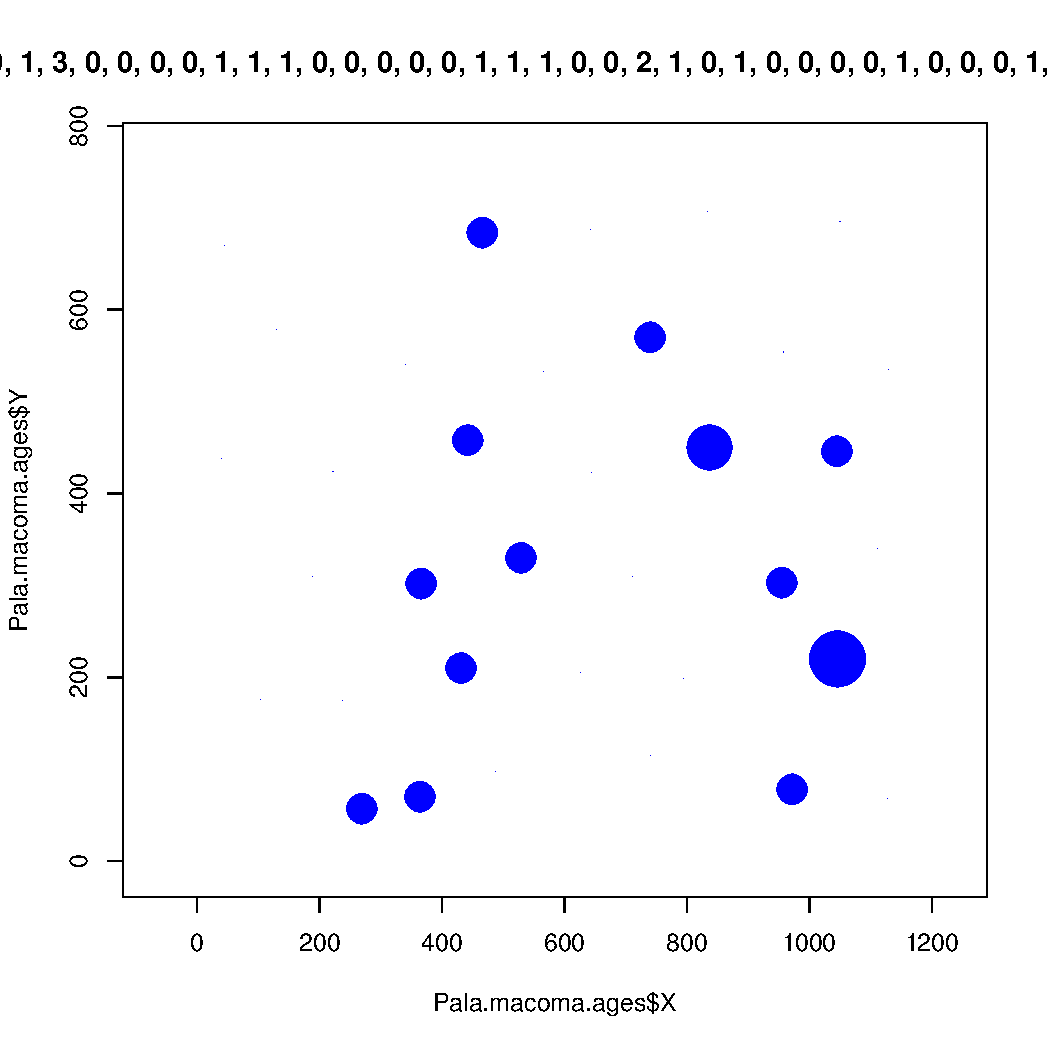
\includegraphics[width=65mm]{../Barenc_Sea/distribution_Moran/Pala_macoma_age_bubb_N12_.pdf}
	\end{center}
	\end{minipage}

	\begin{minipage}[b]{\linewidth}
	\begin{center}
		Моллюски возрастом 13+
	\end{center}
	\end{minipage}

	\begin{minipage}[b]{.46\linewidth}
%Фигурка в первом ряду слева размер отведенный под весь этот объект \textendash 0.46 от ширины строки
%Параметр [b] означает, что выравнивание этих министраниц будет по нижнему краю
	\begin{center}
		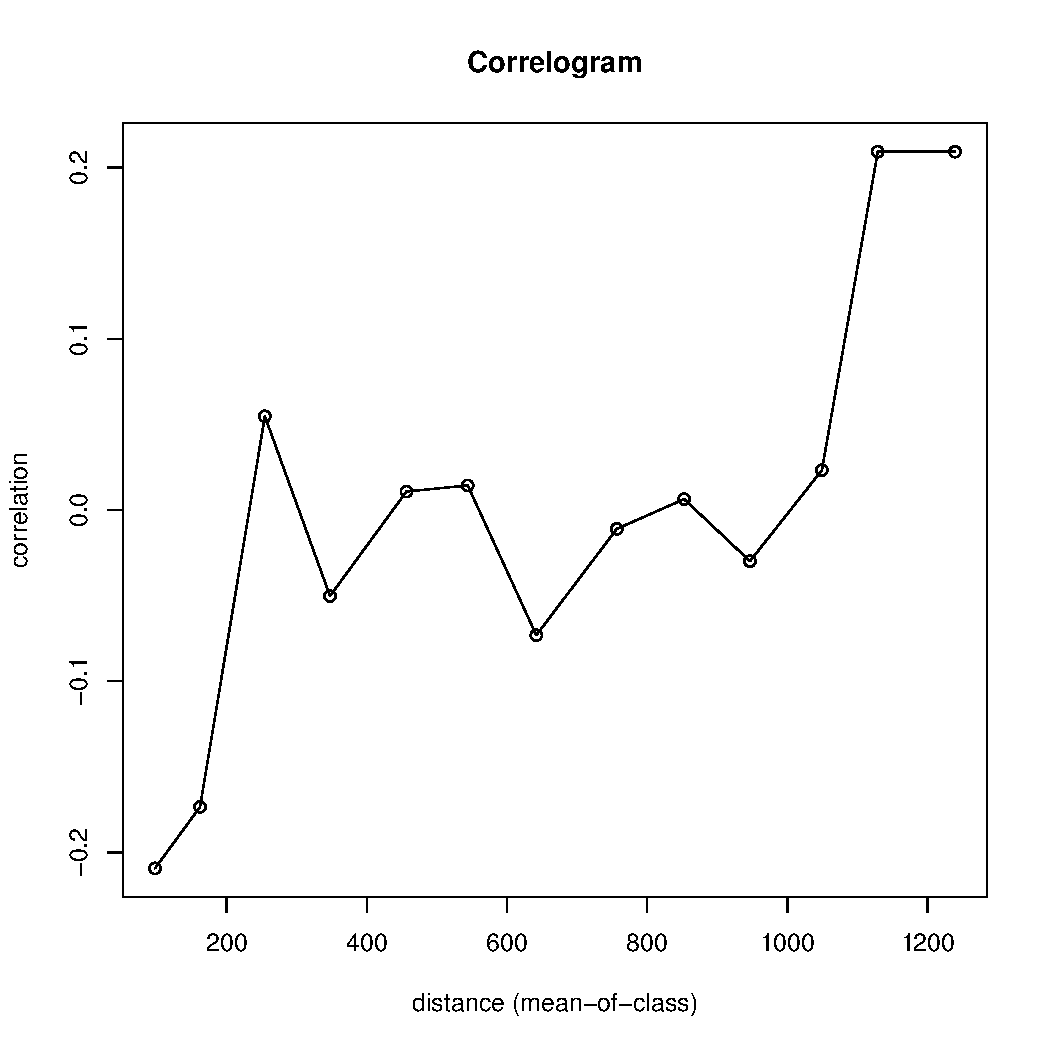
\includegraphics[width=65mm]{../Barenc_Sea/distribution_Moran/Pala_macoma_age_N13_.pdf}
	\end{center}
	\end{minipage}
%
	\hfil %Это пружинка отодвигающая рисунки друг от друга
%
	\begin{minipage}[b]{.46\linewidth}
%Следующий рисунок - первый ряд справа %DUNGEON S_4 \ AB
	\begin{center}
		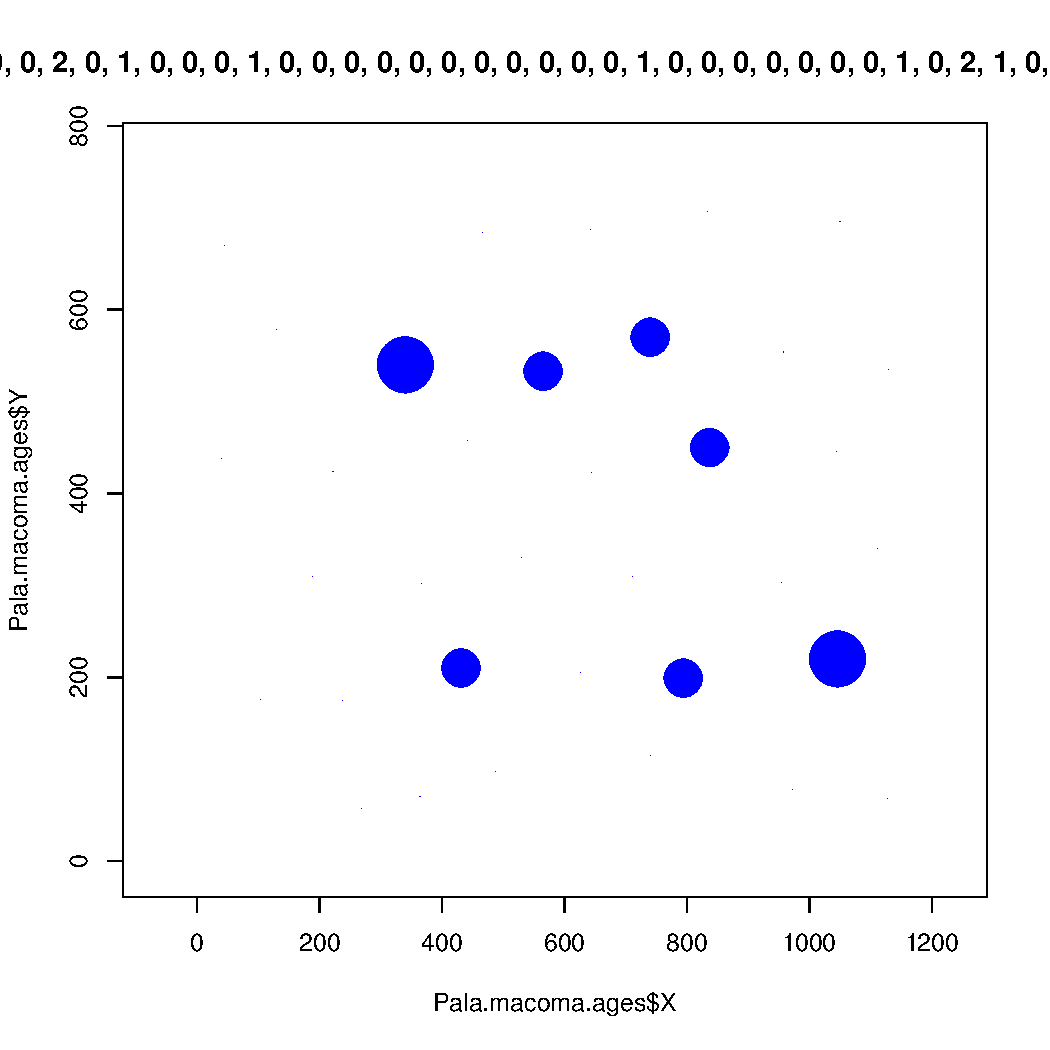
\includegraphics[width=65mm]{../Barenc_Sea/distribution_Moran/Pala_macoma_age_bubb_N13_.pdf}
	\end{center}
	\end{minipage}

	\begin{minipage}[b]{\linewidth}
	\begin{center}
		Моллюски возрастом 14+
	\end{center}
	\end{minipage}
	
	\begin{minipage}[b]{.46\linewidth}
	%Фигурка в первом ряду слева размер отведенный под весь этот объект \textendash 0.46 от ширины строки
	%Параметр [b] означает, что выравнивание этих министраниц будет по нижнему краю
	\begin{center}
%	{\small N~{\it Cerastoderma edule}}
		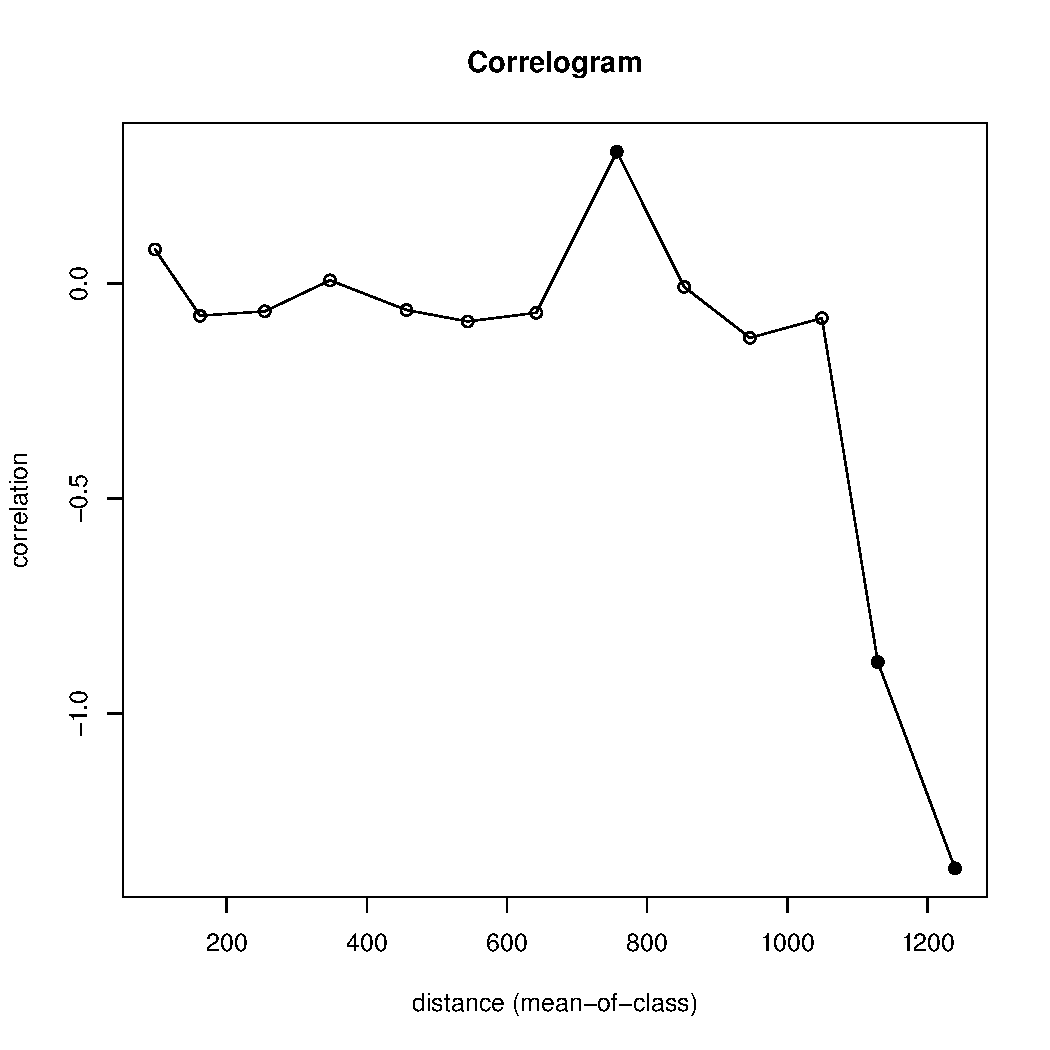
\includegraphics[width=65mm]{../Barenc_Sea/distribution_Moran/Pala_macoma_age_N14_.pdf}
	\end{center}
	\end{minipage}
	%
	\hfil %Это пружинка отодвигающая рисунки друг от друга
	%
	\begin{minipage}[b]{.46\linewidth}
%Следующий рисунок - первый ряд справа %DUNGEON S_4 \ AB
	\begin{center}
		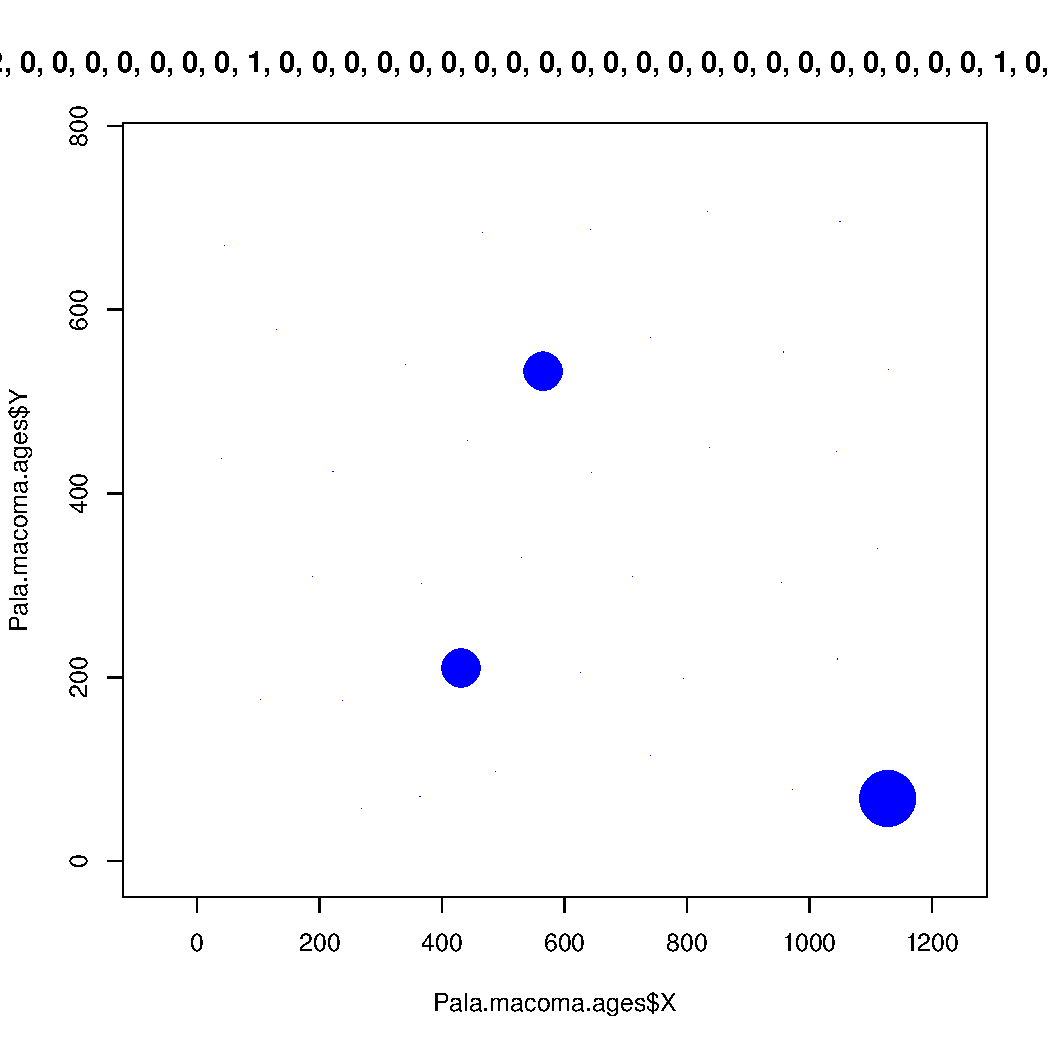
\includegraphics[width=65mm]{../Barenc_Sea/distribution_Moran/Pala_macoma_age_bubb_N14_.pdf}
	\end{center}
	\end{minipage}

%	\caption{Микрораспределение макробентоса на литорали Пала-губы}
%	\label{ris:moransI_Pala}
	\end{figure}
